\documentclass[11pt,a4paper,twoside]{book}
\usepackage{fontenc}[T1]
\usepackage[utf8]{inputenc}
\usepackage[english]{babel}
\usepackage{amssymb,amsmath}
\usepackage[top=2cm,bottom=2cm,left=2cm,right=2cm]{geometry}
\usepackage[pdftex]{graphicx} %per poter inserire le figure
\usepackage{amssymb,amsmath,amsthm,amsfonts}
\usepackage{xspace}
\usepackage{tabularx}
\usepackage{indentfirst}
\usepackage{subfigure}
\usepackage[small]{caption}
\usepackage{eucal}
\usepackage{eso-pic}
\usepackage{url}
\usepackage{booktabs}
\usepackage{afterpage}
\usepackage{parskip}
\usepackage{listings}
\usepackage{fancyhdr}
\usepackage{textcomp}
\usepackage{cite}
\usepackage{multirow}
\usepackage[utf8]{inputenc}   %per riuscire a scrivere gli accenti
\usepackage{setspace}
\usepackage{fancyhdr}
\newenvironment{abstract}{\cleardoublepage\thispagestyle{empty}\null\vfill\begin{center}\bfseries\abstractname\end{center}}{\vfill\null}
\pagestyle{fancy} 


\begin{document}
	\frontmatter
	\begin{titlepage}
		\vspace{5mm}
		\begin{figure}[hbtp]
			\centering
			
\includegraphics[scale=.16]{Logo_unipd.png}
		\end{figure}
		\vspace{5mm}
		\begin{center}
			{{\huge{\textsc{\bf UNIVERSIT\`A DEGLI STUDI DI PADOVA}}}\\}
			\vspace{5mm}
			{\Large{\bf Dipartimento di Fisica e Astronomia ``Galileo Galilei''}} \\
			\vspace{5mm}
			{\Large{\textsc{\bf Master Degree in Physics}}}\\
			\vspace{20mm}
			{\Large{\textsc{\bf Final Dissertation}}}\\
			\vspace{30mm}
			\begin{spacing}{3}
				{\LARGE \textbf{Proibing the Reheating Phase After Inflation}}\\
			\end{spacing}
			\vspace{8mm}
		\end{center}
		
		\vspace{20mm}
		\begin{spacing}{2}
			\begin{tabular}{ l  c  c c c  cc c c c c  l }
				{\Large{\bf Thesis supervisor}} &&&&&&&&&&& {\Large{\bf Candidate}}\\
				{\Large{\bf Prof. Nicola Bartolo}} &&&&&&&&&&& {\Large{\bf Raffaele Giusti}}\\
				{\Large{\bf Thesis co-supervisor}}\\
				{\Large{\bf Prof./Dr. Name Surname}}\\
			\end{tabular}
		\end{spacing}
		\vspace{15 mm}
		
		\begin{center}
			{\Large{\bf Academic Year 2021/2022}}
		\end{center}
	\end{titlepage}
	\clearpage{\pagestyle{empty}\cleardoublepage}

\begin{abstract}
	Inflation is the standard scenario, completely consistent with a variety of data, to understand the  
	generation of primordial scalar (density) perturbations, i.e.  the seeds of all the cosmological structures we  
	see today, and also of tensor perturbations (i.e. primordial gravitational waves). Inflation must come to an  
	end, in order for the universe to be filled in with radiation, and to proceed  through the standard radiation  
	dominated era, during which, e.g. primordial nucleosynthesis can take place. Such a transition (called  
	reheating phase) from the inflationary stage to the standard radiation dominated epoch, is the least known  
	part of the inflationary scenario, because, e.g., it involves couplings of the fields driving inflation to other  
	(relativistic) particles.  
	
	Nonetheless the precision of cosmological data has allowed recently to put already some constraints on  
	such a reheating phase.  
	
	This Thesis will provide an up-to-date review of all the cosmological observables that can be used to open  
	a new window into such period of the early universe. Moreover it will focus on an alternative observational  
	probe that has been investigated recently, namely spatial anisotopies of the energy density of primordial  
	gravitational waves from inflation. The Thesis will explore how such anisotropies depend on, e.g., the  
	equation of state of the Universe during the reheating phase, or e.g., on the number of relativistic degrees  
	of freedom generated during this phase and their thermalisation properties.
\end{abstract}
	
\tableofcontents
	

\chapter{Introduction}

In modern cosmology one of the most important theories is represented by \textit{cosmological inflation}. \\
Inflation was an era during the early hystory of the Universe, before the epoch of primordial nucleosynthesis, during which the Universe expansion was accelerated. Such a period can be attained if the energy density of the Universe is dominated by the vacuum energy density associated with the potential of a scalar field, called the \textit{inflaton field} $ \phi $. \\
Inflation leads to a very rapid expansion of the Universe and can elegantly solve the flatness, the horizon and the monopole problems of the Standard Big Bang Cosmology (indeed, the first model of inflation by Guth in 1981 was introduced to address such problems \cite{Guth:Intro}). It can explain the production of the first density perturbations in the early Universe which are the seeds for the Large Scale Structure (LSS) in the distribution of galaxies and underlying dark matter, and for the Cosmic Microwave Background (CMB) temperature anisotropies that we observe today. Inflation has become the dominant paradigm to understand the initial conditions for structure formation and CMB anisotropies.\\
During this era primordial density fluctuations and gravitational waves are created from quantum fluctuations \textquotedblleft redshifted" out of the horizon during the rapid expansion and here \textquotedblleft frozen\textquotedblright.\\
From this period we can observe temperature anisotropy in the CMB caused by perturbations at the surface of the last scattering. The CMB temperature anisotropies are first detected by the Cosmic Background Explorer (COBE) satellite \cite{COBE1:intro},\cite{COBE2:intro}. \\
Another impressive confirmation of the inflationary theory has been provided by the data of the Wilkinson Microwave Anisotropy Probe (WMAP) mission that has produced a full-sky map of the angular variations of the CMB with unprecedented accuracy. WMAP data confirm the inflationary mechanism as responsible for the generation of superhorizon fluctuations \cite{WMAP:intro}, \cite{NonGauss:Intro}.\\
More recently, the best constraints on the CMB data are provided by the \textit{2018 Planck measurements} \cite{Planck2018:intro}. The \textit{Planck} data have given a very precise characteritation of the primordial cosmological perturbations and have allowed cosmological parameters to be constrained at the sub-percent level. Thus, \textit{Planck} measurements provide  a powerful constraint to inflationary models.\\

The literature contains a large number of different models of inflation. Each model amounts to a choice for the potential  of the inflaton, plus a period of ending inflation, called \textit{reheating}.\\
The main models of inflation focuse on two different paradigms. Throughout the early 1990s discussion was dominated by the \textit{single-field models}. In these models, the scalar field potential often is chosen to be some convenient simple function, such as a monomial or exponential, and the initial conditions are chosen such that the scalar field is well displaced from any minimun.\\
In the mid-1990s, this paradigm was challenged by a new wave of inflationary model building, based on particle physics motivation such as the theories of supersymmetry, supergravity, and superstrings. In such a period we have a new class of models, known generically as \textit{hybrid inflation}, which rely on interactions between two scalar fields and utilize the flat potentials expected in supersymmetry theories \cite{Liddle:intro}. \\
In other scenarios we have the presence of a further scalar field besides the inflation that does not influence the inflationary dynamics (for example the \textit{curvaton scenario}), or the inflaton coupled to a scalar field or a gauge field. Finally, there are theories based on Modified Gravity (MG) that involve a modification of General Relativity \cite{GWFromInflation:Intro}.\\

Inflation cannot proceed forever. In fact, the greatest successes of the Standard Big Bang model, such as primordial nucleosynthesis and the origin of the CMB, require the standard evolution from radiation to matter dominated era.\\ 
The transition from inflation to later stages of the evolution of the Universe (radiation and matter dominance) is referred to as \textit{reheating}. In the simplest models (single-field, slow-roll scenario) inflation ends when the inflaton field starts rolling fast along its potential, it reaches the minimun and then oscilates around it. During reheating the inflaton loses its energy, eventually leading the production of ordinary matter.\\
 More intricate scenarios include non perturbative processes such as (broad) resonance decay, tachyonic instability, instant preheating, fermionic preheating. The \textit{preheating} denotes the initial stage of reheating where we have an exponentially decay that generate high occupation numbers in selected frequency bands.  \\ 
 The aim of this Thesis is provide a complete and up-to-date review of the main models of reheating in the literature.
However, the reheating era is difficult to constrain observationally. In the absence of topological defects like monopoles or strings, the fluctuations produced during reheating remain sub-horizon and cannot leave an observable imprint at the level of the CMB or LSS. A lower bound is placed on the reheating temperature (\textit{i.e}. the temperature at which the standard radiation era of the Universe begins after reheating) by primordial nucleosynthesis (BBN) $ T_{BBN} \sim  10^{-2} Gev $ \cite{Steigman:nucleosynthesisIntro}. The scale of inflation is bounded from above and can be as large as $ \sim 10^{16} Gev $, leaving for the reheating temperature an allowed range of many orders of magnitude. 
Moreover, a variety of signatures relative to production of primordial black holes, magnetic field, unwanted relics, and also to mechanisms such as baryo- and leptogenesis, may be traced back to specific preheating/reheating models \cite{ReheatingPredictionsSingleFieldModel:intro} .\\ 

An extremely important prediction of cosmological inflation is the generation of a Stochastic Background of primordial Gravitational Waves (SGWB). Primordial GW are in fact not expected in the non inflationary standard early-universe models and will provide, if detected, a \textit{smoking gun} probe of inflation. In the standard slow roll inflationary scenario tensor fluctuations of the metric (\textit{i.e} primordial GW) are characterized by a nearly scale invariant spectrum on super-horizon scales. The amplitude of the GW signal is usually described by the tensor-to-scalar ratio \textit{r}, defined as the ratio between the tensor and scalar power spectrum amplitudes at a given pivot scale $ k_{*} $.\\
The current best bound on $ \textit{r} $ comes from the joint analysis of Planck, BICEP2, Keck Array and other data, which yields $ r < 0.07 $ at $ 95 \% $ C.L. for $ k_{*}$ = $ 0.05\ Mpc^{-1} $ \cite{Bicep2:Intro}. \\
A crucial point is that, even in the simplest single field framework, different inflationary scenarios predict different values of r. The study of observational signatures of primordial GW thus provide not only a way to probe the general inflationary theory, but also to discriminate in detail among specific models.\\
A detection of primordial GW would not only be extremely important for Cosmology but also for High Energy and Fundamental Physics. Since the energy scale of inflation is directly linked to the value of the tensor-to-scalar ratio, by means of a detection of $ r $ we would obtain a hint of the the physics beyond the Standard Model and the precise indication of the energy regime of such new physics.\\
Indeed, the primordial GW are the object of a growing experimental effort, and their detection will be a major goal for Cosmology in the forthcoming  decades. \\
The main observational signature of the inflationary GW background is a curl-like pattern (B-mode) in the CMB. A number of, present or forthcoming, ground-based or baloon-borne experiments, are specifically aimed to B-mode detection. Unfortunately, the B-modes measured by BICEP2 \cite{Bicep2BMode:Intro} did not point to any inflationary signal, but several next-generation CMB space missions have been proposed in recent years with the specific goal of B-mode detection such as COrE \cite{COre:intro} or PRISM \cite{PRISM:intro}. 
Finally, we have the possibility of a future direct detection, by experiments such as aLIGO \cite{LIGO:intro}, or eLISA \cite{Lisa:Intro}, especially if some inflationary models produced a blue-tilted primordial tensor spectrum \cite{GWFromInflation:Intro}.\\
In this Thesis we will focus on another type of GW: those generated by classical mechanism during reheating after inflation. By investigating  GW we cannot neglect this stage. In fact, there are many models for the reheating period which provide further GW production, besides that inflationary stage. Moreover, it can be shown that reheating parameters are related to inflationary power-spectra ones, so that the constraints on tensor perturbations are related to those on the reheating period.


In this work we are going to review all the most important inflation and reheating scenarios. After the first two chapters, we will present detailed models of reheating about each of its stages (Preheating, Bubbly Stage, Scalar Wave Turbolence,Thermalitation) investigated in the literature. Moreover, we will review predictions about the production of GW, observable signatures on CMB and the possibility of direct detection of GW from reheating epoch.\\
The Thesis is organized with the following plan:
In the chapter 1 we review the standard single-field model of slow-roll inflation and we derive the physical observables that can be seen and constrained from CMB. \\
In chapter 2 we overview the main inflationary models that are important for the subsequent reheating epoch. Moreover, we present the principal signatures on CMB coming from GWs and reheating parameters. We end this chapter describing a toy model of reheating.\\
In the chapter 3, we investigate about \textit{preheating}, the first stage of reheating, in the model of parametric resonance, and we examinate the GWs generated in this model and observable today. \\
In  chapter 4 we examinate the other important model of preheating: preheating after hybrid inflation. Then, we briefly consider other models of preheating such as fermionic preheating, instant preheating and multi-field reheating.\\
In  chapter 5 and 6 we examinate the subsequent and final stages after preheating: the bubbly stage and thermalitation.\\
In chapter 7 we  overview the principal signatures  of the reheating epoch and we present a new approach to study the reheating epoch that consists in examinating the spatial anisotropies of the energy density of primordial gravitational waves from inflation. 
 
 \mainmatter
 
\chapter{Inflation}

The inflation theory not only provides an excellent way to solve flatness and horizon problems but also generates density perturbations as seeds for large-scale structure in the universe. Quantum fluctuations of the field that drives inflation (called \textit{inflaton}) are streched on large scales by the accelerated expansion. In the simplest version of the single-field scenario the fluctuations are \textquotedblleft frozen" after the scale of perturbations leaves the Hubble radius during inflation. Long after the inflation ends, the perturbations cross inside the Hubble radius again. Thus, inflation provides a causal mechanism for the origin of large-scale structure in the universe. An important prediction of inflation is that density perturbations generally exhibit nearly scale-invariant spectra. This prediction can be directly tested by the measurement of the temperature anisotropies in Cosmic Microwave Background (CMB). Indeed, the anisotropies observed by the Cosmic Background Explorer (COBE) in 1992 showed nearly scale invariant spectra. All data acquired until now have continued to confirm the main predictions of the inflationary theory within observational errors \cite{InflationDynamicsAndReheating:chap1}.\\
In this first chapter we review the simple standard model of slow-roll inflation and we derive observables and relations that will be used in the next chapters.

\section{Standard Big-Bang Cosmology}

The standard big-bang cosmology is based upon the cosmological principle which requires that the universe is homogeneous and isotropic on averaging over large volumes.\\
A homogeneous and isotropic universe is described by the Friedmann-Robertson-Walker metric (FRW):

\begin{equation}
	\label{metric}	
	ds^{2}   = - dt^{2} + a^{2}(t)\Big[\frac{dr^{2}}{1-Kr^{2}}  +  r^{2}(d\theta^{2} + sin^{2} \theta d\phi^{2})\Big] . 
\end{equation}
Here $a(t)$ is the scale factor with $ t $ being the cosmic time and $(r,\theta,\phi) $ are comoving (spherical) coordinates. The constant $ K $ is the spatial curvature, where positive, zero, and negative values correspond to closed, flat, and hyperbolic spatial sections respectevely. \\
The evolution of the universe is dependent on the material within it. A key role is played by the \textit{equation of state} relating the energy density $ \rho (t) $ and the pressure $ P(t) $. Assuming a perfect and barotropic fluid we can describe it with the relation $ P=\omega\rho $ with $ \omega=0 $ for non-relativistic matter (dust) and $ \omega=1/3 $ for radiation.
For example in the universe we have $ P=0 $ or $ P=1/3 $ if it is dominated by dust or radiation, respectevely. \\
The dynamical evolution of the universe is known once we solve the Einstein equations for General Relativity:

\begin{equation}
	\label{eq:gr}
	G_{\mu\nu}  = R_{\mu\nu} - \frac{1}{2}g_{\mu\nu}R=8\pi G T_{\mu\nu}
\end{equation}

where $ G_{\mu\nu} $ is the Einstein Tensor, $ R_{\mu\nu} $, $ R $, $ T_{\mu\nu}$, and G are the Ricci tensor, Ricci scalar, energy-momentum tensor and gravitational constant, respectively. The energy momentum tensor $ T_{\mu\nu} $ describes the perfect fluid with density energy $ \rho $ and isotropic pressure P that fills the universe.\\
The Planck energy, $m_{pl}=1.2211 \times 10^{19}$ GeV, is related to G through the relation $ m_{pl} = (\hslash c^{5}/G)^{1/2}$. Hereafter we use the units $ \hslash = c = 1 $.\\
From the Einstein equations (\ref{eq:gr}) for the background FRW metric (\ref{metric}), we obtain the Friedmann Equations:
\begin{equation}
	\label{friedmannEquations1}
	H^{2}=\frac{8\pi G}{3}\rho - \frac{K}{a^{2}},
\end{equation}
\begin{equation}
	\label{friedmannEquations2}	
	\frac{\ddot{a}}{a} = -\frac{4\pi G}{3}(\rho + 3P),
\end{equation}

where the dots denote the derivative with respect to t, and $ H=\dot{a}/a $ is the Hubble expansion rate. Combining these relations we obtain the energy conservation equation 

\begin{equation}
	\label{energyCons}
	\dot{\rho} + 3H(\rho + P)=0,
\end{equation}

which is known as the continuity or fluid equation.\\
The Friedmann equation (\ref{friedmannEquations1}) can be rewritten as 

\begin{equation}
	\label{densityParameter}
	\Omega - 1 = \frac{K}{a^{2}H^{2}}
\end{equation}

where 

\begin{equation}
	\label{criticalDensity}
	\Omega=\frac{\rho}{\rho_{c}}, \quad    with \quad   \rho_{c}=\frac{3H^{2}}{8\pi G}
\end{equation}

where the density parameter $ \Omega $ is the ratio of the energy density to the critical density $ \rho_{c} $.\\
When the spatial geometry is flat (K=0, $ \Omega $=1) the solution for equations (\ref{friedmannEquations1})
and (\ref{friedmannEquations2}) are $ a \propto t^{1/2} \quad  (\rho \propto a^{-4}) $ for the radiation dominated era, and $ a\propto t^{2/3} \quad  (  \rho \propto  a^{-3}$) for dust dominated era.\\
Thus, from these equations we obtain a decelerate expansion ($ \ddot{a} < 0 $) for the universe.\\

\section{Standard cosmology and inflation}
In this section we briefly review the problems with the standard cosmology and how are solved by the idea of inflation \cite{Liddle:intro},\cite{Dodelson:Chap1}, \cite{InflationDynamicsAndReheating:chap1}. 

\subsection*{\emph{Flatness problem}}
In the standard big-bang theory with $ \ddot{a} < 0  $, the $ a^{2}H^{2} (= \dot{a}^{2}) $ term in (\ref{densityParameter}) always deacreases. This means that
$ \Omega $ tends to evolve away from unity with the expansion of the universe. Howewer, since present observations suggest that $ \Omega  $ is within a few percent of unity today, $ \Omega $ is forced to be much closer to unity in the past. For example, we require $ |\Omega-1| < \mathcal{O}(10^{-16}) $ at the epoch of nucleosynthesis and  $ |\Omega-1| < \mathcal{O}(10^{-64}) $ at the Planck epoch \cite{Liddle:intro}. This appears an extreme and innatural fine-tuning of initial conditions. Unless initial conditions are chosen  very accurately, the universe either collapses too soon, or expands too quickly before the structure can be formed. This is the so-called \textit{flatness problem}.

\subsection*{\emph{Horizon problem}}
Consider a comoving wavelength, $ \lambda $, and the corresponding physical wavelength, $ a\lambda $, which at some time is inside the Hubble radius, $ H^{-1} $ (\emph{i.e. a$ \lambda \leq  H^{-1}  $}). The standard big-bang cosmology is characterized by the cosmic evolution of  $a \propto t^{n} $ with 0 $< n < 1$. In this case the physical wavelength grows as $ a\lambda \propto t^{n} $, whereas the Hubble radius evolves as $H^{-1}\propto t$ . Therefore the physical wavelength becomes much smaller than the Hubble radius at late times.
This means that a causally connected region can only be a small fraction of the Hubble radius.\\
For example if we observe photons in the cosmic microwave background (CMB) which are last-scattered at the time of decoupling turns out that the causally connected regions on the surface of last scattering corresponds to an angle of order 1°.\\
This appears to be in contrast with observations of the CMB which has the same temperature to high precision in all directions on the sky. There is no way to establish thermal equilibrium if these points were never been in causal contact before last scattering. This is the so-called \textit{horizon problem} .

\subsection*{\emph{Large-scale structure}}
Experiments which observe temperature anisotropies in the CMB find that the amplitude of the anisotopies is small and their power spectrum is close to scale-invariant on large scales. It is impossible to generate such fluctuations  via causal processes in a FRW metric in the time between the big bang and the time of the last scattering.

\subsection*{\emph{Relic density problem}}
In Particle Physics the standard paradigm to study the fundamental interactions is the Spontaneous Symmetry Breaking (SSB) of gauge symmetries.\\
In the early universe the breaking of such symmetries leads to the production of many unwanted relics such as monopoles, cosmic strings, and other topological defects \cite{TopDefects:Linde}. For example, any grand unified theory based on a simple Lie group that includes the U(1) of electromagnetism must produce monopoles. String theories also predict supersymmetric particles such as gravitinos, Kaluza-Klein particles, and moduli fields.\\
If these massive particles exist in the early stages of the universe and they are stable (or sufficiently long-lived) could become the dominant matter in the early universe depending on their number density and therefore contradict a variety of observation such as those of the light element abundances. This problem is known as the \textit{relic density problem}.

\subsection*{\emph{The idea of inflation}}

The problems in the standard big bang cosmology lie in the fact that the universe always exhibits decelerated expansion. Instead, let us assume  the existence of a stage in the early universe with an accelerated expansion: 

\begin{equation}
	\label{acc.expansion}
		\ddot{a} > 0
\end{equation}

From the relation (\ref{friedmannEquations2}) this gives the condition

\begin{equation}
	\label{equationOfState}
	\rho + 3P < 0
\end{equation}

and, from  the equation of state $ P = \omega \rho  $, we obtain 

\begin{equation}
	\label{w parameter}
	\omega < -\frac{1}{3}
\end{equation}

The condition (\ref{acc.expansion}) essentialy means that $ \dot{a}\ (= aH) $ increases during inflation and hence that the comoving Hubble radius, $ (aH)^{-1} $, decreases in the inflationary phase.

\subsubsection*{\textit{Flatness problem}}
Since the $ a^{2}H^{2} $ term in (\ref{densityParameter}) increases during inflation, $ \Omega $ is rapidly driven towards unity. After the inflationary period ends, the evolution of the universe is followed by the conventional big-bang phase and $|\Omega-1| $ begins to increase again. As long as the inflationary expansion lasts sufficiently long and drives $ \Omega $ very close to one, $ \Omega $  will remain close to unity even in the present epoch.  

\subsubsection*{\textit{Horizon problem}}
Since the scale factor evolves approximately as $ a \propto t^{n} $ with n $ > 1 $ during inflation, the physical wavelength, $a \lambda $, grows faster than the Hubble radius, $ H^{-1}(\propto t)$. Therefore, physical wavelenghts are pushed outside the Hubble radius during inflation and then causally connected regions can be much larger than the Hubble radius, thus potentially solving the horizon problem.\\
A detailed computation shows this is achieved when the universe expands at least about $ e^{70} $ times during inflation, or 70 e-folds of expansion \cite{Liddle:intro}.

\subsubsection*{\textit{Large-scale structure}}
The inflationary period leads to perturbations of the scalar field that drives inflation and then of the energy density of the universe. In the early stage of inflation the scales of these perturbations are well within the Hubble radius and causal physics can works generating small quantum fluctuations. During the later stages these scales are pushed outside the Hubble radius (\textit{i.e.} the first Hubble radius crossing). Fluctuations of the scalar field become over-damped on long-wavelengths and the perturbations can be described as classical on these large scales. After the inflationary period these scales of perturbations  cross inside the Hubble radius again (\textit{i.e.} the second Hubble radius crosssing).\\
The small perturbations imprinted during inflation have amplitudes determined by the Hubble rate which is approximatevely constant during this period and hence  leads to an almost scale-invariant spectrum with constant amplitude on different scales.\\
In this way the inflation naturally provides a causal mechanism to generate the seeds of density perturbations observed in the CMB anisotropies.

\subsubsection*{\textit{Relic density problem}}
During the inflationary phase the energy density of massive particles scales as $ a^{-3} $, much faster than the energy density  of the universe (considering $ a \propto t^{n} $ with $ n>1 $, we have $ H \propto t^{-1} \propto a^{-1/n}$ that leads $  \rho \propto a^{-2/n} $). Thus, these particles are red-shifted away during inflation, solving the monopole problem.

\section{The inflaton equation}
As we have seen  from (\ref{w parameter}) a period of inflation is possible if the pressure $ P $ is negative with 

\begin{equation}
\label{Pressure-density}
P < -\frac{\rho}{3}
\end{equation}

In the special case in which $ \omega = -1 $ ($P=-\rho$) we have a period in the hystory of the universe called \textit{de Sitter stage}. \\
Such a period can be obtained inserting a cosmological constant $ \Lambda $ in the Einstein Equations: 

\begin{equation}
	\label{RGModified}
	R_{\mu\nu} - \frac{1}{2}g_{\mu\nu}R = 8\pi G T_{\mu\nu} - \Lambda g_{\mu\nu}.
\end{equation}

Considering the energy continuity equation (\ref{energyCons}) and the first Friedmann equation (\ref{friedmannEquations1}) we see that in a de Sitter phase $ \rho = constant $ and $ H = H_{inf} \simeq constant $ (we neglect the curvature K which is soon redshifted away as $ a^{-2} $).\\
Solving the second Friedmann equation (\ref{friedmannEquations2}) we obtain an exponentially growing of the scale factor

\begin{equation}
	\label{scaleFactorDeSitter}
	a(t)=a_{i} e^{ H_{inf}(t-t_{i})}	
\end{equation}

where $t_{i}$ is the time at which inflation starts. \\
The cosmological constant can be interpreted as the energy of the quantum vacuum state of the system, the \textit{vacuum} energy density contributed by any particle species. Even if it is simple to have such exponentially expansion of the universe the inflation must end at some point. Thus, there must be some dynamics regulating such system.\\
We can obtain this if we consider a scalar field, called the \textit{inflaton}, that dominates the energy in this epoch and leads the expansion.\\

Consider in full generality the total action

\begin{equation}
	\label{totalAction}
	S^{TOT} = S_{HE} + S_{\phi} + S_{m} 
		        = \frac{1}{16\pi G} \int d^{4} x \sqrt{-g} (R + \mathcal{L} [\phi , \partial_{\mu} \phi ] + \mathcal{L}_{matter}) 	
\end{equation}

where $ g $ is the determinant of the metric tensor $ g_{\mu\nu} $, $ S_{HE} $ is the Hilbert-Einstein action, $ S_{\phi} $ is the inflaton scalar field action and $ S_{m} $ is the action of the rest of the matter besides the inflaton (fermions, gauge fields, other scalars...). We will neglect $ S_{m} $ because, in general, they are subdominant at early times. \\
The action for a minimally-coupled real scalar field $ \phi $ is given by

\begin{equation}
	\label{actionScalarField}
	S=\int d^{4} x \sqrt{-g} \mathcal{L} = \Big [-\dfrac{1}{2} g^{\mu\nu} \partial_{\mu}\phi \partial_{\nu} \phi - V(\phi)\Big]	
\end{equation}

where $ V(\phi) $ specifies the scalar field potential and  can have different forms depending on the model. For example it can be a simple quadratic potential $ V(\phi)=\frac{1}{2}m^{2}\phi^{2} $, with $ m $ the mass of the particle associated to $ \phi $,$  $ or can describes  self interactions $ V(\phi) = \frac{\lambda}{4} \phi^{4} $. $ V(\phi) $ can represent also interactions of $ \phi $ with other fields and contains quantum radiative corrections. \\

To characterize the evolution of the scalar field in an expanding universe we can associate to $ \phi $ its stress-energy momentum $ T_{\mu\nu} $, which in General Relativity is given from a generic lagrangian by

\begin{equation}
	\label{stressEnergyMomentum}
	T_{\mu\nu}= \frac{-2}{\sqrt{-g}}\frac{\delta S}{\delta g^{\mu\nu}}=
	\frac{-2}{\sqrt{-g}}\Big [-\frac{\partial (\sqrt{-g} \mathcal{L})}{\partial g^{\mu\nu}} + \partial _{\alpha} \frac{\partial (\sqrt{-g} \mathcal{L})}{\partial \partial_{\alpha} g^{\mu\nu}} + ... \Big ].
\end{equation}

Assuming a minimally-coupled field (\textit{i.e.} doesn't involve direct coupling with gravity, e.g. $ \varepsilon  \phi^{2} R$ terms), the stress-energy tensor assumes the form

\begin{equation}
	\label{tensorScalrField2}
	T^{\phi}_{\mu\nu} = -2 \frac{\partial \mathcal{L}_{\phi}}{\partial g^{\mu\nu}} + g^{\mu\nu} \mathcal{L}_{\phi}
 =\partial_{\mu} \phi \partial_{\nu} \phi + g_{\mu\nu} \Big [-\frac{1}{2}g^{\mu\nu}\partial_{\mu}\phi\partial_{\nu}\phi - V(\phi)\Big]
\end{equation}

The equation of motion for $ \phi $ is derived by varying the action (\ref{actionScalarField}) with respect $ \phi $ obtaining the Klein-Gordon equation

\begin{equation}
	\label{KGEquation}
	\square  \phi = \frac{\partial V}{\partial \phi}	
\end{equation}

where $\square$ is the covariant D'Alembert operator

\begin{equation}
	\label{alembertOperator}
	\square \phi = \frac{1}{\sqrt{-g}}\partial_{\nu}\Big (\sqrt{-g} g^{\mu\nu} \partial_{\mu}\phi\Big ).
\end{equation}

In a FRW universe described by the metric (\ref{metric}), the evolution equation for $ \phi $ becomes

\begin{equation}
	\label{eomForPhi}	
	\ddot{\phi} + 3H\dot{\phi} - \frac{\nabla^{2} \phi}{a^{2}} + V'(\phi)=0
\end{equation}

where $ V'(\phi)=dV/d\phi $. Through $ 3H\dot{\phi} $ the field "feels" a friction due to the expansion of the universe, which will play a crucial role.\\

We can now express the inflaton field $ \phi $ as the sum of the classical background value and the field fluctuations

\begin{equation}
	\label{splitInflaton}
	\phi(t,\textbf{x})=\phi_{0}(t) + \delta \phi(t,\textbf{x})
\end{equation}

where $\phi_{0}(t) =\ <0|\phi(t,\textbf{x})|0> $  is the classical field, that is the expectation value of the inflaton field on the initial isotropic and homogeneous state, while $\delta \phi (t,\textbf{x})$ represents the quantum fluctuations around $ \phi_{0}(t)$.
We will consider first the background dynamics and then the evolution of quantum perturbations during inflation. This separation is justified by the fact that quantum fluctuations are much smaller than the classical value and therefore negligible when looking at the classical evolution.

\section{Classical Dynamics}
The inflaton field $ \phi(t) $  behaves like a perfect flud with background energy density and pressure given by 

\begin{equation}
	\label{energyDensityPressure}
	T^{0}_{0} = -\Big [\dfrac{1}{2} \dot{\phi}^{2}_{0}(t) + V(\phi_{0}) \Big ] = -\rho_{\phi}(t)
\end{equation}
\begin{equation*}
	T^{i}_{j} = -\Big [\dfrac{1}{2} \dot{\phi}^{2}_{0}(t) - V(\phi_{0}) \Big ]\delta^{i}_{j} = \delta^{i}_{j} P_{\phi} (t)	
\end{equation*}

where $ \rho_{\phi} (t) $ is the energy density and $ P_{\phi} (t) $ the isotropic pressure. $ T_{\mu\nu} $ is diagonal and the spatial part is the same in every direction as a consequence of isotropy and homogeneity resulting in a tensor typical of perfect fluids. Hereafter we don't insert the subscript \textquotedblleft 0" when we denote the background field. \\
Therefore if 

\begin{equation}
	\label{conditionFlatPotential}
	V(\phi) \gg \frac{1}{2} \dot{\phi}^{2}
\end{equation}

we see that 

\begin{equation}
	\label{deSitterCondition}
	P_{\phi} \simeq -\rho_{\phi}
\end{equation}

which gives rise to a quasi-de-Sitter phase.\\
From this simple calculation we realize that a scalar field whose energy is dominant in the universe and whose potential energy dominates over the kinetic term gives inflation. The condition (\ref{conditionFlatPotential}) is called \textit{slow-roll} regime, during which $ V(\phi) \simeq constant $ provides accelerated expansion driven by the vacuum energy density of $ \phi $, which mimics an effective cosmological constant $ \Lambda $.\\
The ordinary matter fields, in the form of a radiation fluid, and the spatial curvature K are usually neglected during inflation because their contribution to the energy density is redshifted away during the accelerated expansion.
\begin{figure}
	\centering
	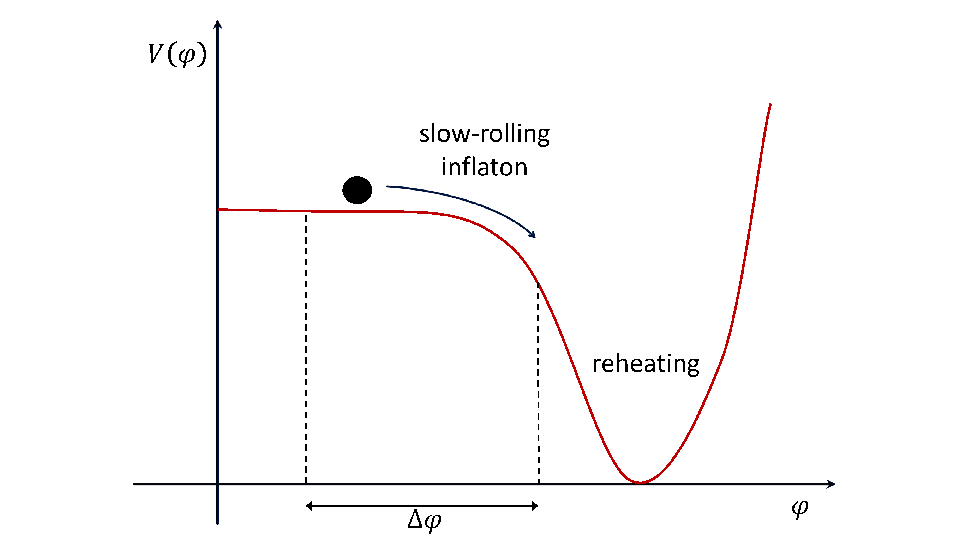
\includegraphics[width=0.65\linewidth, height=0.25\textheight]{Images/Chap1/GWFromInflation_Fig1}
	\caption{Example of inflationary potential with a flat region. After the slow-roll of the inflaton field $\phi$, the reheating phase starts. The field oscillates around the minimum of the potential and decays in other particles. $\Delta$ $\phi$ indicates the inflaton excursion between the horizon exit of a comoving scale and the end of inflation \cite{GWFromInflation:Intro}. }
	\label{fig:gwfrominflationfig1}
\end{figure}

\subsection{Slow-roll parameters}

We quantify now under which circumstances a scalar field may give rise to a period of inflation.
Considering the background scalar field $ \phi $ (homogeneous and isotropic) the equation of motion (\ref{eomForPhi}) becomes

\begin{equation}
	\label{eomHomogeneousField}
	\ddot{\phi} + 3H \dot{\phi} + V'(\phi) = 0.
\end{equation}

If the \textit{slow-roll} condition $ \phi^{2} \ll V(\phi) $ is satisfied, the scalar field slowly rolls down its potential. Such a period can be achieved if the inflaton field is in a region where the potential is sufficiently flat. Since the potential is flat we may also expect that $\ddot{\phi}$ is negligible as well. We will assume this is true and we will quantify this condition.\\
Requiring the slow-roll condition the Friedmann equation (\ref{friedmannEquations1}) becomes 

\begin{equation}
	\label{friedMannEqDuringInflation}
	H^{2} \simeq \frac{8\pi G}{3} V(\phi),
\end{equation}

where we assumed that the inflaton field dominates the energy density of the universe. Moreover, assuming also $\ddot{\phi}$ negligible we obtain the new equation of motion

\begin{equation}
	\label{newEQMphiDotDotNegligible}
	3H\dot{\phi} = -V'(\phi)
\end{equation}

Using (\ref{newEQMphiDotDotNegligible}) and the slow-roll condition (\ref{conditionFlatPotential}) we obtain

\begin{equation}
	\label{condition1}
	\frac{(V')^{2}}{V} \ll H^{2}
\end{equation}

and, considering $\ddot{\phi} \ll 3H\dot{\phi}$,

\begin{equation}
	\label{condition2}
V'' \ll H^{2}	.
\end{equation}

These two conditions represent the flatness conditions of the potential which are conveniently parametrized in terms of the so-called \textit{slow-roll parameters}.
The slow-roll parameters quantify the slow-roll regime dynamics in order to give predictions of specific models and to compare it with others and with observations.\\
Firstly, we define the $\epsilon$ parameter

\begin{equation}
	\label{epsilon}
	\epsilon = - \frac{\dot{H}}{H^{2}}
\end{equation}

that describes how much $ H $ changes during inflation.
To relate this variable to the slow-roll relation $ \dot{\phi}^{2} \ll V(\phi) $ let us derive the first Friedmann equation (neglecting the curvature)

\begin{equation}
	\label{derivingEpsilon1}
	H^{2}=\frac{8\pi G}{3}\rho_{\phi} = \frac{8\pi G}{3} \Big (\frac{1}{2}\dot{\phi}^{2} + V(\phi) \Big )
\end{equation}

obtaining,

\begin{equation}
	\label{FriedmannDerived}
	2H\dot{H} = \frac{8\pi G}{3} \Big (\dot{\phi} \ddot{\phi} + V'(\phi)\dot{\phi} \Big ).
\end{equation}
Now, inserting the equation of motion of the inflaton $ \ddot{\phi} = -3H\dot{\phi} - V'  $ in (\ref{FriedmannDerived}) we obtain

\begin{equation}
	\label{Hdot}
	\dot{H} = -4\pi G\dot{\phi}^{2}
\end{equation}

Finally, using $ H^{2}=(8\pi G/3)V(\phi) $  

\begin{equation}
	\label{epsilon2}
	\epsilon= - \frac{\dot{H}}{H^{2}}=4\pi G \frac{\dot{\phi}^{2}}{H^{2}} \simeq \frac{3}{2} \frac{\dot{\phi}^{2}}{V(\phi)}
\end{equation}

where the last equality si valid only in the slow-roll regime. Therefore, we can interpret $\epsilon$ as the ratio between the kinetic energy and the potential. \\
Hence assuming $ V(\phi) \gg \dot{\phi}^{2}  $ we obtain 

\begin{equation}
	\label{conditionEpsilon}
	\epsilon \ll 1 .
\end{equation}
Moreover, exploiting $ H\dot{\phi} \simeq -V' $, we can write

\begin{equation}
	\label{newEpsilon}
	\epsilon=4\pi G \frac{\dot{\phi}^{2}}{H^{2}} \simeq \frac{1}{16\pi G} \Big (\frac{V'}{V} \Big )^{2}	
\end{equation}

which means that if $\epsilon \ll 1 $ , $V'$ is small and the potential is flat. Thus, $\epsilon$ quantifies the flatness of the potential.\\

Considering the second slow-roll condition $ \ddot{\phi} \ll 3H\dot{\phi} $, we can define the second slow-roll parameter as 

\begin{equation}
	\label{etaParameter}
	\eta = - \frac{\ddot{\phi}}{H\dot{\phi}} \ll 1
\end{equation}

As we have done for $\epsilon$ we can relate this expression to the potential. To do this we can derive $ \dot{\phi} \simeq -V'/3H $, obtaining

\begin{equation}
	\label{phiDerivedEtaParameter}
	\ddot{\phi} = -\frac{V'' \dot{\phi}}{3H} + \frac{\dot{H}}{3H^{2}}V'.
\end{equation}
Plugging this into the definition of $\eta$ we obtain

\begin{equation}
	\label{eta2}
	\eta \simeq \frac{V''}{3H^{2}} - \frac{\dot{H}}{H^{2}}\frac{V'}{3H\dot{\phi}} \simeq \eta_{V} - \epsilon
\end{equation}

where $ \frac{V'}{3H\dot{\phi}} \simeq -1 $ and we have defined $ \eta_{V}=\frac{V''}{3H^{2}} $. Thus again, having $\eta \ll 1$ means to have a flat potential.\\

A successful period of inflation requires that $ \epsilon, |\eta| \ll 1 $. Moreover, exists a hierarchy of slow-roll parameters: for example, one can define the slow-roll parameter related to the third derivative of the potential

\begin{equation}
	\label{secondOrderParameter}
	\xi^{2} = \Big (\frac{1}{4\pi G} \Big )^{2} \Big (\frac{V'V'''}{V^{2}}\Big )
\end{equation}

which is a second order slow-roll parameter. The third derivative of the potential corresponds to an eventual self-interaction of the inflaton field. \\
One can use these parameters with the data collected from observations to reconstruct the shape of the potential.\\
At first-order in the slow-roll parameters $\epsilon$ and $\eta$ can be considered constant, since the potential is very flat and their derivatives are higher orders in these parameters. In fact it is easy to see that $ \dot{\epsilon},\dot{\eta} = \mathcal{O}(\epsilon^{2},\eta^{2}) $.\\

If we written $ \epsilon = - \dot{H}/H^{2} $ we can notice that

\begin{equation}
	\label{scaleFactorParameter}
	\ddot{a}=\dot{\dot{a}}=\dot{(aH)}=\dot{a}H + a\dot{H}=aH^{2}\Big (1+\frac{\dot{H}}{H^{2}}\Big ) = aH^{2}(1-\epsilon) .
\end{equation} 

Thus, inflation can be attained only if $\epsilon < 1$. As soon as this condition fails, inflation ends.\\
This condition alone can be sufficient to realise inflation. However, having also $\eta \ll 1 $  assure that inflation lasts for long enough. In fact, $ \eta = - \frac{\ddot{\phi}}{H\dot{\phi}}  \ll 1 $ both ensures that inflation is an attractor solution and that $\dot{\phi}$ remains constant and small for long enough. In other worlds, $\eta$ controls the duration of inflation.\\

Despite the semplicity of the inflationary theory, the number of inflationary models that have been proposed so far is enormous, differing for the kind of potential and for the underlying particle phyisics theory. In the second chapter we will discuss about the most important models, but we just to mention here that the main classification in connection with the observations is the one in which the single-field inflationary models are divided into three broad groups as \textquotedblleft small field", \textquotedblleft large field" (or chaotic) and \textquotedblleft hybrid" type, according to the region occupied in the ($\epsilon$ - $\eta$) space by a given inflationary potential.\\

\section{Inflation and cosmological perturbations}
The description of the universe as a perfectly homogeneous and isotropic FRW model is an idealitation. Actually, we are interested in deviations from homogeneity and isotropy that enable us to characterise different models.\\
So far we have considered only the dynamics of a homogenous scalar field driving inflation. But to investigate inflation models in more detail and to test theoretical predictions against cosmological observations we need to consider inhomogeneous perturbations. \\
Besides the background inflationary dynamics, we have the evolution of the quantum fluctuactions of the inflaton field $ \delta\phi(t,\textbf{x}) $. In the inflationary model there are primordial energy density perturbations, associated with these vacuum fluctuations, which survive after inflation and are the origin of all the structures in the universe.\\
Once the universe became matter dominated ($ z \simeq 3200 $) primeval density inhomogeneites ($ \delta \rho/\rho \simeq 10^{-5} $) were amplified by gravity and grew into the structure we see today. The existence of these inhomogeneities was in fact confirmed by the COBE discovery of CMB anisotropies.\\
In this section we summarise how the quantum fluctuations of a generic scalar field evolve during an inflationary stage. For more details see \cite{Liddle:intro},\cite{NonGauss:Intro},\cite{Dodelson:Chap1}.

\subsection{Quantum Fluctuations}
Consider for semplicity a scalar field $ \phi $ (the inflaton) with an effective potential $ V(\phi) $ in a pure de Sitter stage, during which the Hubble rate $ H $ is constant. 
We first split the field $ \phi(\tau,\textbf{x}) $ in the homogeoneous classical part, $ \phi(\tau) $, and its fluctuations $ \delta\phi(\tau,\textbf{x}) $

\begin{equation}
	\label{splitInflatonTau}
	\phi(\tau,\textbf{x})=\phi(\tau) + \delta \phi(\tau,\textbf{x})
\end{equation}

where $ \tau $ is the conformal time, related to the cosmic time $ t $ through $ d\tau=dt/a(t) $.\\
We consider the Fourier transform of the fluctuations
\begin{equation}
\label{fourierTransform}
\delta\phi(\tau,\textbf{x})=\frac{1}{(2\pi)^{3}}\int d^{3}k e^{i \textbf{k}\cdot\textbf{x}}\delta\phi(\tau,k).
\end{equation}
Redefining  the scalar field as 
\begin{equation}
\label{fieldRedefinition}
\widetilde{\delta \phi}	= a\delta\phi
\end{equation}
 we can promote it to an operator which can be decomposed as 
 \begin{equation}
 	\label{quantitation}
 	\widetilde{\delta \phi}(\tau,\textbf{x})=\int \frac{d^{3} \textbf{k}}{(2\pi)^{3/2}} \big[u_{k}(\tau)a_{\textbf{k}}e^{i \textbf{k}\cdot\textbf{x}} + u_{k}^{*}(\tau)a_{\textbf{k}}^{\dagger}e^{-i \textbf{k}\cdot\textbf{x}}\big]
 \end{equation}
 
 where we have introduced the creation and annihilation operators $ a_{\textbf{k}} $ and $ a^{\dagger}_{\textbf{k}} $.\\
 The creation and annihilation operators for $\widetilde{\phi}$ satisfy the standard commutation relations
 \begin{equation}
 	\label{commutationRelations}
 \big[a_{\textbf{k}},a_{\textbf{k}'}] = 0, \qquad \big[a_{\textbf{k}},a_{\textbf{k}'}^{\dagger}] = \delta^{(3)}(\textbf{k}-\textbf{k}')
 \end{equation}
and the modes $ u_{k}(\tau) $ are normalized so that they satisfy the condition

\begin{equation}
	\label{normalitation}
	u^{\ast}_{k} u_{k}' - u_{k} u'^{\ast}_{k} = -i,
\end{equation}
where primes denote derivatives with respect to the conformal time $ \tau $. \\
Expanding the equation of motion for the scalar field (\ref{eomForPhi}) in the fluctuations $\delta\phi(\tau,\textbf{x})$ in Fourier space we obtain
\begin{equation}
	\label{eomFluctuations}
	u''_{k}(\tau) + \Big[k^{2} - \frac{a''}{a} + \frac{\partial^{2} V}{\partial\phi^{2}}a^{2}\Big] u_{k}(\tau) = 0.
\end{equation}

 where $ m^{2}_{\phi} = \partial^{2} V / \partial\phi^{2} $ is the effective mass of the scalar field. This equation describes an harmonic oscillator with a frequency changing in time, due to the expansion of the universe.\\
 The modes $ u_{k}(\tau) $ at very short distances must reproduce the form for the ordinary flat space-time quantum field theory. Thus, well within the horizon, in the limit $ k/aH \rightarrow \infty $, the modes should approach plane waves of the form
 
 \begin{equation}
 	\label{planeWave}
 	u_{k}(\tau) \rightarrow \frac{1}{\sqrt{2k}}e^{-ik\tau}.
 \end{equation}

Let us consider a special case where the inflaton is massless in a pure de-Sitter universe ($m_{\phi} = 0, H=constant $). In this situation the equation (\ref{eomFluctuations}) becomes
\begin{equation}
\label{eomMasslessDesitter}
u''_{k}(\tau) + \Big[k^{2} - \frac{a''}{a}\Big]u_{k}(\tau) = 0.
\end{equation}

Using $a d\tau=dt$, and $ a \propto e^{Ht}$ in a de-Sitter stage 
\begin{equation}
	\label{horizon}
	\frac{a''}{a}= \frac{2}{\tau^{2}}=2a^{2}H^{2}=\frac{2}{r_{H}^{2}}
\end{equation}
where $ r_{H} $ is the comoving Hubble radius.\\
Thus, we can study (\ref{eomMasslessDesitter}) in two different regimes: the \textit{sub-horizon} regime where $ \lambda_{phys} \ll H^{-1} $, $ k^{2} \gg a^{2}H^{2} \simeq a''/a $, and the \textit{super-horizon} regime where $ \lambda_{phys} \gg H^{-1} $, $ k^{2} \ll a^{2}H^{2} \simeq a''/a $.\\
In the sub-horizon case the equation of motion reduces to the wave equation

\begin{equation}
\label{waveEquationFluctuation}
u''_{k} + k^{2}u_{k}=0\  \rightarrow\  u_{k}(\tau)= \frac{1}{\sqrt{2k}}e^{-ik\tau} 
\end{equation}

and the field,

\begin{equation}
	\label{fieldSubHorizon}
	 \delta\phi_{k}=u_{k}/a=\frac{1}{a}\frac{1}{\sqrt{2k}}e^{-ik\tau}
\end{equation}

from which we can notice that it has a decreasing amplitude $ |\delta\phi| = 1/a\sqrt{2k} $, which depends on the inverse of $ a $.
In the super-horizon regime we obtain the equation

\begin{equation}
	\label{superHorizon}
	u''_{k} + \frac{a''}{a}u_{k}=0.
\end{equation}

This equation is solved by

\begin{equation}
	\label{solutionSuperHorizon}
	u_{k}(\tau) = B(k)a(\tau) + A(k)a^{-2}(\tau)
\end{equation}
where A, B are integration constants in $ \tau $ which depends on $ k $. In term of the field we get
\begin{equation}
	\delta\phi_{k} = B(k) + A(k)a^{-3}(\tau) \simeq B(k) = constant,
\end{equation}
where we have neglected the decaying term which gets washed away by inflation.\\
We can fix the amplitude of the growing mode, $ B(k) $, by matching the (absolute value of) this solution to the plane wave solution (\ref{fieldSubHorizon}) when the fluctuation with wavenumber k leaves the horizon ($ k = aH $)
\begin{equation}
	|B(k)|= \frac{1}{a\sqrt{2k}} = \frac{H}{\sqrt{2k^{3}}},
\end{equation}
So that the quantum fluctuations of the original scalar field $ \phi $ on super-horizon scales are constant,
\begin{equation}
	\label{frozenField}
	|\delta \phi_{k}| = \frac{|u_{k}|}{a} = \frac{H}{\sqrt{2k^{3}}}.
\end{equation}

From this simple computation we can see that inflation is able to provide a mechanism to generate density perturbations (and gravitational waves). To understand what is going on, a key ingredient is the decreasing with time of the comoving Hubble horizon $ (aH)^{-1} $ during inflation. The wavelength of a quantum fluctuation in the inflaton field soon exceeds the Hubble radius. The quantum fluctuations arise on scales which are much smaller than the comoving Hubble radius, which is the scale beyond which causal processes cannot operate. On small scales we can use the usual flat space quantum field theory to describe the scalar field vacuum fluctuations.\\
However, the inflationary expansion \textit{stretches} the wavelength of these fluctuations to outside the horizon. The quantum fluctuations of the inflaton are amplified (and frozen) on super-horizon scale, resulting in a net number of scalar field particles.\\
On large scales the perturbations just follow a classical evolution. Since microscopic physics does not affect the evolution of fluctuations when their wavelengths are outside the horizon, the amplitude of these inhomogeneites are "frozen" and fixed at some nonzero value $ \delta\phi $ at the horizon crossing.\\
The amplitude of the fluctuations on super-horizon scales then remains almost unchanged for a very long time, whereas the wavelength grows exponentially. Thus, these frozen fluctuations of the inflaton are equivalent to the appearance of a classical field $ \delta\phi $ that does not vanish after having averaged over some macroscopic interval of time. Moreover, the same mechanism also generates a stochastic background of gravitational waves.\\
The quantum fluctuations of the inflaton generate also fluctuations in the space-time metric, giving rise to perturbations of the curvature $ \mathcal{R} $. On super-horizon scales, curvature fluctuations are frozen in and considered as classical.\\
When the wavelength of these perturbations reenters the horizon, in the radiation or matter dominated epoch, the curvature perturbations of the space-time give rise to matter (and temperature) perturbations $ \delta \rho $ via the Poisson equation.\\
These fluctuations will then start growing, giving rise to the structure we observe today.

\subsection{Power spectrum}

To characterise the properties  of a perturbation field we introduce the \textit{power spectrum}.\\
Consider a random field $ f(t,\textbf{x}) $ that can be expanded in Fourier space as 
\begin{equation}
\label{fourierTransform}
	f(t,\textbf{x}) = \int \frac{d^{3}\textbf{k}}{(2\pi)^{3/2}} e^{i\textbf{k}\cdot \textbf{x}} f_{\textbf{k}}(t).
\end{equation}

The power spectrum $ P_{f}(k) $ can be defined by means the relation
\begin{equation}
\label{powerSpectrum}
\big<f_{\textbf{k}_{1}}f^{*}_{\textbf{k}_{2}}\big> \equiv \frac{2\pi^{2}}{k^{3}}P_{f}(k) \delta^{(3)}(\textbf{k}_{1}-\textbf{k}_{2})
\end{equation}
where the angled brackets denote the ensemble average. The power spectrum measures the amplitude of the fluctuations at a given scale $k$. Indeed, if we consider the last definition the mean square value of $f(t,\textbf{x})$ in real space is
\begin{equation}
\label{meanSquare}	
\big<f^{2}(t,\textbf{x})\big>= \int \frac{dk}{k} P_{f}(k).
\end{equation}

To describe the slope of the power spectrum  we define the $ \textit{spectral index}$   $n_{f}(k)$
\begin{equation}
\label{spectralIndex}
n_{f}(k) - 1 \equiv \frac{d \ lnP_{f}}{d \ ln k}.
\end{equation}  

For the inflaton field quantum fluctuations $ |\delta \phi_{k}| = \frac{|u_{k}|}{a} $,

\begin{equation}
	\label{fluctuations}
	\big < \delta\phi_{\textbf{k}_{1}}, \delta \phi^{*}_{\textbf{k}_{2}}\big>=\frac{2\pi^{2}}{k^{3}}|\delta \phi_{\textbf{k}_{1}}| \delta^{(3)}(\textbf{k}_{1}-\textbf{k}_{2}).
\end{equation}

Therefore,
\begin{equation}
\label{spectrumFluctuation}
P_{\delta \phi}(k) = \frac{k^{3}}{2\pi^{2}}|\delta \phi_{k}|^{2},		
\end{equation}

with $ \delta \phi_{k} \equiv u_{k}/a $.	

\subsection{Exact solution}
Now we briefly recap how to solve exactly the equation of motion for the modes $ u_{k} $ (\ref{eomFluctuations}). This equation can be rewritten in the form of \textit{Bessel equation} 
\begin{equation}
	\label{bessel}
	u''_{k}(\tau) + \Big[k^{2} - \frac{\nu^{2}-1/4}{\tau^{2}}\Big] u_{k}(\tau)=0.
\end{equation}
In this form, it is equivalent to the Bessel equation
\begin{equation}
	z^{2}y''(z) + zy'(z) + (z^{2}-\nu^{2})y(z)=0.
\end{equation}				
whose solutions are known to be of the form 
\begin{equation}
	\label{solutionPerturbations}
	u_{k}(\tau) = \sqrt{-\tau}\big [c_{1}(k)H^{(1)}_{\nu}(-k\tau) + c_{2}(k)H_{\nu}^{(2)}(-k\tau)].
\end{equation}
where $ H^{(1)}_{\nu} $ and $ H^{(2)}_{\nu} $ are the Henkel functions of first and second kind, respectively.
The parameter $ \nu $ can be expressed in terms of the slow roll parameters.\\
In the case of a quasi De-Sitter universe and  (little) massive scalar field we have the relation $ 3/2 - \nu \simeq \eta_{V} - \epsilon$.
 The requirement  of a light mass is due to the fact that if $ m^{2}_{\phi} \ge H^{2}$,  $ \delta \phi_{k} $ remains in the vacuum state and fluctuations get suppressed. From now we omit the subscript \textquotedblleft $V$" in $\eta$.\\
If we impose  that in the ultraviolet regime $ k \gg aH $ $ (-k\tau \gg 1) $ the solution matches the plane-wave solution $ e^{-ik\tau}/\sqrt{2k} $ that we expect in flat space-time. Knowing the asymptotic beheaviour of the Hankel functions on sub-horizon scales

\begin{equation}
\label{Hankel1}
H^{(1)}_{\nu}(x \gg 1) \sim \sqrt{\frac{2}{\pi x}} e^{i(x-\frac{\pi}{2}\nu-\frac{\pi}{4})} ,
\quad
H^{(2)}_{\nu}(x \gg 1) \sim \sqrt{\frac{2}{\pi x}} e^{-i(x-\frac{\pi}{2}\nu-\frac{\pi}{4})}
\end{equation}

and on super-horizon scales,

\begin{equation}
\label{Hankel2}
H^{((1)}_{\nu}(x \ll 1) \sim \sqrt{\frac{2}{\pi}}e^{-i\frac{\pi}{2}}2^{\nu-\frac{3}{2}}\frac{\Gamma(\nu)}{\Gamma(3/2)}x^{-\nu}	
\end{equation}

we can set in (\ref{solutionPerturbations})  $ c_{2}(k)=0 $ and $ c_{1}(k)=\frac{\sqrt{\pi}}{2}e^{i(\nu + \frac{1}{2})\frac{\pi}{2}} $.\\
We finally obtain for the fluctuations $ |\delta \phi_{k}| $ 
\begin{equation}
	\label{solutionDeltaPhi}
	|\delta \phi_{k}|= \frac{H}{\sqrt{2 k^{3}}}\Big (\frac{k}{aH}\Big)^{\frac{3}{2}-\nu},
\end{equation}

yielding for the power spectrum (\ref{spectrumFluctuation})

\begin{equation}
	\label{PowerSpectrumperturbation}
	P_{\delta \phi}(k) = \Big (\frac{H}{2\pi}\Big)^{2}\Big (\frac{k}{aH}\Big)^{3-2\nu}
\end{equation}

where $ \nu $ is given by $ 3/2 - \nu \simeq \eta_{V} - \epsilon$.\\
In the power spectrum just computed there is an inconsistency. In the computation the scalar field is perturbed on a unperturbed spacetime. Thus, we should also include perturbations of the metric to have a correct result. To do so, we need to consider scalar perturbations of the metric and use gauge invariant quantities. But before doing that, we are going to consider the tensorial perturbations of the metric: the gravitational waves.

\subsection{Gravitational waves}
Inflation predicts the existence of a scale invariant spectrum of primordial gravitational waves, sourced by the same quantum fluctuations described in the previous sections. Gravitational waves are only weakly coupled to matter fields, and move freely through the universe from the moment they are produced.\\
The perturbations of the inflaton field will induce perturbations of the metric. This leads to a stochastic background of gravitational waves (GW)  which are represented by tensor perturbations of the metric.\\
A stochastic background of waves is a continuos set of waves, fully characterized  only by their global statistic properties. It consists of a signal coming from every direction in the sky. It is different from the signals coming from astrophysical sources (merging neutron stars,  binary black holes...), which come from a specific direction in the sky. \\
In this section we explain how inflation can generate this stochastic background. 

We start considering the perturbed spatially flat FLRW metric, where we neglect scalar and vector perturbations,
\begin{equation}
	ds^{2} = -dt^{2} + a^{2}(t)[\delta_{ij} + h_{ij}]dx_{i}dx_{j}
\end{equation}
with $ h_{ij} $, in the so called Transvere-Traceless gauge (TT gauge), are such that
\begin{equation}
	h_{ij}=h_{ji} \qquad h^{i}_{i}=0 \qquad h^{i}_{j|i} = 0.
\end{equation}
 
 At linear level Einstein's equations for $ h_{ij} $ are 
 \begin{equation}
 	\ddot{h}_{ij} + 3H\dot{h}_{ij} - \frac{\nabla^{2}h_{ij}}{a^{2}}= \Pi^{TT}_{ij}
 \end{equation}
where $\Pi^{TT}_{ij}$ is a tensor, with the same properties of $ h_{ij} $, which is a source term coming from possible anisotropic stress of the matter source. It is related  to the last term of the stress-energy tensor of a perfect fluid $ T_{\mu\nu} = (\rho + P)u_{\mu}u_{\nu} + Pg_{\mu\nu} + \Pi_{\mu\nu}$, called anisotropic stress tensor, which can get a contribution in the case of astrophysical sources when we have a non vanishing quadrupole moment. We will see that this term is also important to describe the gravitational waves emitted in the reheating phase.\\
However, at first order, it is vanishing during single field inflation and the equation of $ h_{ij} $ becomes 
\begin{equation}
	\label{eqh}
		\ddot{h}_{ij} + 3H\dot{h}_{ij} - \frac{\nabla^{2}h_{ij}}{a^{2}}=0,
\end{equation}
which is similar to the equation for the quantum vacuum fluctuation in the case of a massless scalar field.\\
Since there is no source term, GWs are the intrinsic quantum fluctuations of the metric. Moreover, they provide a \textit{smoking gun} of inflation and would be the first ever detected evidence of quantum gravity.\\
The equation (\ref{eqh}) describes the evolution of the tensor $ h_{ij} $, which has 2 independent DOF, corresponding to the two possible polaritations of GWs $ \lambda = (+,\times) $. Such object can be decomposed in Fourier space as 

\begin{equation}
	\label{fouriewrh}
	h_{ij}(\tau,\textbf{x}) = \sum_{+\times} \int \frac{d^{3} k}{(2\pi)^{3}}e^{i\textbf{k}\cdot \textbf{x}}h_{\lambda}(\textbf{k},\tau)\epsilon^{\lambda}_{ij}(\textbf{k})
\end{equation}
where $ \epsilon^{\lambda}_{ij}(\textbf{k}) $ are the polaritation tensors, which satisfy
\begin{equation}
	\epsilon_{ij}=\epsilon_{ji} \qquad \epsilon^{i}_{i}=0 \qquad  k^{i}\epsilon_{ij}(\textbf{k}) =0
\end{equation}
 with normalitation conditions
 \begin{equation}
 \epsilon_{ij}^{\lambda}(\textbf{k})\epsilon^{*ij}_{\lambda'}(\textbf{k})=\delta_{\lambda\lambda'}
 \qquad
 \big (\epsilon_{ij}^{\lambda}(\textbf{k})\big)^{*} = \epsilon_{ij}^{\lambda}(-\textbf{k}).
 \end{equation}
Considering a plane monochromatic gravitational wave propagating in the $\hat{z}$ direction, in Fourier space we have

\begin{equation}
	\epsilon^{+}_{ij} = 
	\begin{pmatrix}
		1 & 0 \\
		0 & -1
	\end{pmatrix}
\qquad
\epsilon^{\times}_{ij} = 
\begin{pmatrix}
	0 & 1 \\
	1 & 0
\end{pmatrix}
\end{equation}
\begin{equation}
	h_{ij}(\textbf{k},\tau) = h_{+}(\textbf{k},\tau)\epsilon_{ij}^{+}(\textbf{k}) + 
	h_{\times}(\textbf{k},\tau)\epsilon_{ij}^{\times}(\textbf{k})
\end{equation}

and, the tensor $ h_{ij} $ satisfies

\begin{equation}
	\ddot{h}_{\lambda} + 3H\dot{h}_{\lambda}+ k^{2}\frac{h_{\lambda}}{a^{2}}=0
\end{equation}
which is the same for each polaritation state.\\
On super-horizon scales, $ k\ll aH $, the solution for $ h_{+,\times} $ is given by a constant plus a decaying mode. Using the canonical normalitation
\begin{equation}
|h_{+,\times}|= \sqrt{32\pi G}|\phi_{+,\times}| = \sqrt{32\pi G} \frac{H}{\sqrt{2k^{3}}}\Big (\frac{k}{aH}\Big)^{-\epsilon}.
\end{equation}
On sub horizon scales ($ k \gg aH $), $ h_{+,\times}=\frac{e^{-ik\tau}}{a(\tau)} $.\\
For the power spectrum we obtain
\begin{equation}
\label{spectumGW}
P_{T}(k)=\frac{k^{3}}{2\pi^{2}}<h^{*}_{ij}h^{ij}>=\frac{16}{M_{pl}^{2}}\Big(\frac{H}{2\pi}\Big )^{2}\Big (\frac{k}{aH}\Big)^{-2\epsilon}
\end{equation}   
where $ H $ indicates the Hubble rate during inflation and we have summed the two polaritations $ (+,\times) $.\\
Therefore we can define the spectral index of inflationary gravitational waves as
\begin{equation}
n_{T} = \frac{d\ ln P_{T}}{d\ ln k} = -2\epsilon.
\end{equation}
In the simplest models one has $ \epsilon > 0 $ so $ n_{T} $ is always red- tilted (on smaller scales the amplitude decreases).
Since during inflation $P_{T} $ $\sim$ $ H^{2} $ and $ H^{2} \simeq \frac{V}{M^{2}_{pl}} $, detecting the tensor spectrum would give us the energy scale of inflation ($ E_{inf} \simeq V^{1/4} $, see later). 

\subsection{Primordial curvature perturbation}
In the standard slow-roll inflationary models the fluctuations of the inflaton field are responsible for the curvature perturbations.
 As said, they are (nearly) frozen on super-horizon scales. When they reenters the horizon lead to pertubations of matter that give rise the structure we see today.\\
To characterise the scalar and curvature perturbations we need gauge invariant quantities.
A complete treatment of this argument is in \cite{NonGauss:Intro}. Here we just summarise the main points.


Consider the perturbed FRW metric at first order including only scalar perturbation and expressed with the conformal time $ \tau=\int dt/a(t) $
\begin{equation}
\label{metricPerturbed}
ds^{2}=a^{2}(\tau) \big [-(1+2\Psi)d\tau^{2} + (1-2\Phi)\delta_{ij}dx_{i}dx_{j} \big]
\end{equation}

The first gauge invariant quantity we consider is
\begin{equation}
	\label{zeta}
	-\zeta \equiv \hat{\Phi} + \mathcal{H}\frac{\delta \rho}{\rho'}
\end{equation}
where $\mathcal{H} \equiv a'/a$ is the Hubble parameter in conformal time and the prime denote differentiation w.r.t it. $\hat{\Phi}$ is referred to as the \textit{curvature perturbation}. This quantity, however, is not gauge invariant since it changes under a transformation on costant time hyper-surfaces $\tau$ $\rightarrow$ $ \tau + \alpha $. Instead, combining the $\hat{\Phi}$ transformation and the gauge transformation for scalars comes out that $\zeta$ in (\ref{zeta}) is gauge invariant. This quantity is called \textit{gauge-invariant curvature perturbation of the uniform energy-density hypersurfaces}.\\
To obtain the $\zeta$ power spectrum consider another gauge invariant quantity called \textit{curvature perturbation on comoving hyper-surfaces}. In the case of a stress-energy tensor of a single scalar field it reads
\begin{equation}
	\label{R}
	\mathcal{R} \equiv \hat{\Phi} + \frac{\mathcal{H}}{\phi'}\delta \phi
\end{equation}

The comoving curvature perturbation $\mathcal{R}$ is related to the curvature perturbation $\zeta$ by
\begin{equation}
	- \zeta = \mathcal{R} + \frac{2\rho}{9(\rho + P)} \Big (\frac{k}{aH}\Big)^{2}\Psi,
\end{equation}
where $\psi$ is the perturbation that appears in the metric. 
From this relation we obtain that on large scales $\mathcal{R} \simeq -\zeta$.\\
In the previous sections we obtained the power spectrum of  the primordial fluctuations of the inflaton (\ref{PowerSpectrumperturbation}). However, we computed it without taking into account the perturbation of the metric.\\
To do so, we define a new gauge-invariant quantity called  \textit{Sasaki-Mukhanov variable}
\begin{equation}
	\label{sasaki-mukhanov}
	\mathcal{Q}_{\phi} \equiv \delta \phi + \frac{\phi'}{\mathcal{H}}\Phi 
\end{equation}
Introducing the field $\tilde{\mathcal{Q}}_{\phi}=aQ_{\phi}$, the Klein-Gordon equation reads \cite{NonGauss:Intro}
\begin{equation}
	\label{finalEOM}
\tilde{\mathcal{Q}}'' + \Big (k^{2} - \frac{a''}{a} + \mathcal{M}_{\phi}^{2}a^{2}\Big)\tilde{\mathcal{Q}}_{\phi} = 0
\end{equation} 
where 
\begin{equation}
 \mathcal{M}^{2}_{\phi}=\frac{\partial^{2} V}{\partial \phi^{2}} - \frac{8\pi G}{a^{3}}\Big (\frac{a^{3}}{H}\dot{\phi}^{2}\Big)
\end{equation}
is an effective mass of the inflaton field. At lowest orders in the slow-roll parameters the latter expression reduces to $ \mathcal{M}^{2}_{\phi}/H^{2} = 3\eta-6\epsilon $. Solving (\ref{finalEOM}) by means of the Hankel functions, as we did in the previous sections, we obtain at super-horizon scales and at  lowest order in the slow-roll parameters the complete solution
\begin{equation}
	\label{solutionPerturbation}
	|Q_{\phi}(k)| = \frac{H}{\sqrt{2k^{3}}}\Big (\frac{k}{aH}\Big)^{3/2-\nu}
\end{equation}
where $ \nu \simeq 3/2 + 3\epsilon - \eta $.\\
This solution leads a power spectrum
\begin{equation}
\label{PSQ}
P_{\mathcal{Q}}=\Big (\frac{H}{2\pi} \Big)^{2}\Big(\frac{k}{aH}\Big)^{3-2\nu}.
\end{equation}
Now, returning to the gauge-invariant curvature perturbation $ \mathcal{R} $ (\ref{R}), we can easily express it in function of the Sasaki-Mukhanov variable. Using (\ref{sasaki-mukhanov}) results
\begin{equation}
	\label{expressionR}
	\mathcal{R}=\dfrac{\mathcal{H}Q_{\phi}}{\phi'} = \frac{H Q_{\phi}}{\dot{\phi}}
\end{equation}
where we have express $ \mathcal{R} $ in terms of the cosmic time.
Finally, using (\ref{PSQ}), we obtain the power spectrum of the curvature perturbation $\mathcal{R}$:
\begin{equation}
\label{PR}
P_{\mathcal{R}}=\Big (\frac{H}{\dot{\phi}}\Big)^{2}P_{\mathcal{Q}}= \Big (\frac{H^{2}}{2\pi \dot{\phi}}\Big)^{2}\Big(\frac{k}{aH}\Big)^{3-2\nu} \simeq \Big(\frac{H^{2}}{2\pi\dot{\phi}}\Big)^{2}_{*}
\end{equation}
where  the asterisk denotes quantities evaluated at the epoch a given perturbation mode leaves the horizon during inflation, that is $ k=aH $.\\
The last equation shows that the curvature perturbations remains  time-independent on super-horizon scales. In the \textit{uniform curvature gauge}, where $ \Phi=0 $, we have $ \zeta \simeq - \mathcal{H}\delta \rho/\rho' $. So, we can connect the inflaton perturbations to observable quantities.
The solution obtained for $\zeta$ is valid  throughout the differen evolution eras of the Universe until the mode remains super horizon.\\
From (\ref{PR}) we can easily obtain the spectral index of the curvature perturbation (at lowest order in the slow-roll approximation)
\begin{equation}
\label{spectralIndex}
n_{\mathcal{R}}-1\equiv \frac{d\ ln P_{\mathcal{R}}}{d\ ln k} = 3 - 2\nu=-6\epsilon + 2\eta.
\end{equation}
Inflationary models predict a power spectrum od density perturbations very close to 1. The specific case in which $ n_{s}=1 $ is called \textit{Harrison-Zel'dovich} spectrum that means that the amplitude of the inflaton pertubations does not depend on the cosmological scale.\\ 
The curvature mode is the quantity which allows to connect the primordial perturbations produced during inflation to the observables.
This result comes from the fact that in single-field slow roll models the intrinsic entropy perturbation of the inflaton field is negligible on large scales. This result holds also during the reheating phase after inflation\cite{NonGauss:Intro}. 

\subsection{Consistency relation}
In the single-field models a important consistency relation holds. To derive it, we introduce the \textit{tensor-to-scalar ratio}
\begin{equation}
\label{tensorScalarRatio}
r(k_{*})\equiv \frac{P_{T}(k_{*})}{P_{S}(k_{*})}
\end{equation}
that yields  the amplitude of the GW with respect to that of the scalar perturbations at some pivot scale $ k_{*} $.\\
We can rewrite the power spectrum $ P_{\mathcal{R}} $ in (\ref{PR}) as function of the slow-roll parameters using the fact that $ \epsilon=-\dot{H}/H^{2}=4\pi G\dot{\phi^{2}}/H^{2} $:
\begin{equation}
	\label{PSRelatedToEpsilon}
P_{\mathcal{R}}(k)=\frac{1}{2M_{P}^{2}\epsilon}\Big (\frac{H}{2\pi}\Big)^{2}\Big (\frac{k}{aH}\Big)^{n_{\mathcal{R}}-1}	
\end{equation}
that yields $ r=16\epsilon $.\\
Furthermore, we have shown that a nearly scale-invariant spectrum of tensor modes is expected, being $ n_{T}=-2\epsilon $. Therefore at the lowest order in the slow-roll parameters, one finds the consistency relation
\begin{equation}
	\label{consistencyRelation}
	r=-8n_{T}
\end{equation}
This equality can be proved only with a measure of the tensor power spectrum (not only the amplitude, but also  its spectral index \textit{i.e.} its shape).\\
Since a large spectral index would invalidate the consistency relation, it will be very hard to measure any scale dependance of the tensors assuming the consistency relation valid.\\
At present we have only an upper bound on the tensor-to-scalar ratio from the joint analysis of BICEP2, Keck Array data and Planck: $ r_{0.05}<0.07 $ at  95$\% $ C.L. \cite{Bicep2:Intro}, assuming valid the consistency relation. The subscript indicates the pivot scale in $ Mpc^{-1} $ units.\\

Finally we can connect the energy scale of inflation to the tensor-to-scalar ration $ r $.\\
From $ H^{2}=8\pi GV/3 = V/3M_{pl}^{2}$ we can link the energy scale of inflation, at the time when the pivot scale leaves the horizon, directly to the parameter $\epsilon$ using (\ref{PSRelatedToEpsilon})
\begin{equation}
	V=24\pi^{2}M_{pl}^{4}P_{\mathcal{R}}\epsilon =(3\pi^{2}P_{\mathcal{R}}/2)M_{pl}^{4}r.
\end{equation}
Thus, considering  the scalar amplitude estimated  by the Planck Collaboration \cite{Plank2015:Chap1} one gets  the following relation between the energy scale of inflation at the time when the pivot scale leaves the Hubble radius, and the tensor-to-scalar ratio:
\begin{equation}
	\label{energyScaleInflation-r}
	V=(1.88\times10^{16}GeV)^{4}\frac{r}{0.10}.
\end{equation}
Then we have a direct link between $ r $ and the energy scale of inflation.\\

In the next chapter we'll overview the most important models of inflation and we'll introduce the important stage of reheating by means a pertubative toy model.\\
The reheating phase is the main focus of this work since it leads very intersting effects and physics. Moreover, the gravitational waves generated by reheating are very different from those generated by inflation and could be detected by future experiments providing a observational window of such period.

\chapter{Inflation Zoology and Reheating}
So far we have not discussed the form of the inflaton potential, $ V(\phi) $. A simple model of inflation was proposed by Guth in 1981 to solve the horizon and flatness problems discussed in the first chapter \cite{Guth:Intro}.
In this model, called  \textit{Old Inflation} scenario, the inflaton is initially trapped in a metastable false vacuum during inflation. Subsequently  it moves towards the true vacuum via a first-order transition. In this scenario inflation is then an exponential expansion of the universe in the supercooled false vacuum state that makes the universe very big and very flat. However, as pointed out by Guth in the paper, this type of inflation produces a random nucleation of bubbles that lead a highly inhomogeneous universe.\\
This problem is solved by the \textit{New Inflation} in 1981-1982 \cite{Chap2: Linde_NewInflation} . In this model, inflation may begin either in the false vacuum, or in an unstable state at the top of the effective potential. Then the inflaton field slowly rolls down to the minimun of the  potential. However, the useful part of inflation responsible for the homogeneity of the universe does not occur in the false vacuum state in this model. Unfortunately, also this picture has problems. It works only if the effective potential of the field $ \phi $ has a very flat plateau near $\phi=0$, which is somewhat artificial. Moreover, in most versions of this scenario the inflaton field  has an extremelly small coupling constant, so it could not be in thermal equilibrium  with other matter fields.\\
In the beginning of the 80's, on the basis of all available observations (CMB, abundance of light elements) everybody believed that the universe instead was in a state of thermal equilibrium from the very beginning and the stage of inflation was just an intermediate stage of the evolution of the universe.\\
In the 1983 the \textit{Chaotic Inflation} resolved all problems of old and new inflation \cite{ChaoticInflationLinde:Chap2}. According to this scenario, inflation may begin even if there was no thermal equilibrium in the early universe and it may occur in the scenarios with simplest quadratic potential. Moreover, it is not limited to theories with polynomial potentials: chaotic inflation occurs in any theory where the potential has a sufficiently flat region, which allows the existence of the slow-roll regime, as described in the previous chapter. A review of the hystory of inflation can be found in \cite{Chap2:Linde_HystoryInflation}.  \\
The different kinds of single-field inflationary models can be classified in the following way. The first class consists of the \textit{large field} models, in which the initial value of the inflaton is large and it slowly rolls down toward  the potential minimum at smaller $\phi$. Chaotic inflation is one of the representative models of this class. The second class consists of the \textit{small fied} models, in which the inflaton field is small initially and slowly evolves toward the potential minimum at larger $\phi$. An example of this type is new inflation. The third class consists of the \textit{hybrid inflation} models, in which inflation typically ends by a phase transition triggered by the presence of a second scalar field.\\
Several models of inflation can involve a coupling with gauge fields or other scalar fields. These models are very interesting because they can give rise to a source of gravitational waves and curvature perturbations \cite{GWFromInflation:Intro}. \\
The main reheating models discussed in the literature are concentrated on the end of inflation in the chaotic and hybrid scenarios. Thus, in the first part of this chapter we review these important models. In the second part  we start to focus on the main topic of this work: the reheating phase. We'll start considering an elementary, simple scenario of reheating. From chapter 4 we'll see that, instead, reheating models have very complicate and non-linear dynamics. 

\section{Inflationary models}
\subsection{Guth's Inflation}
We start from the Guth model of inflation because it contains very interesting points such as entropy production and the random nucleation of bubbles, phenomena that also occurs in non-linear stages of reheating \cite{Guth:Intro}.\\
This model was introduced to solve the horizon and flatness problem: initially, in fact, the early universe was assumed to be highly homogeneous, despite to the fact that separated regions were causally disconnected, and the initial value of the Hubble constant had to be extremelly fine-tuned to produce the flat universe we see today.\\
In this scenario the universe is assumed to be homogeneous and isotropic and then is described by the Robertson-Walker metric, that we rewrite:

\begin{equation}
	\label{metricCh2}	
	ds^{2}   = - dt^{2} + a^{2}(t)\Big[\frac{dr^{2}}{1-kr^{2}}  +  r^{2}(d\theta^{2} + sin^{2} \theta d\phi^{2})\Big] . 
\end{equation}

where $ k=+1,-1,0 $ denotes a closed, open, or flat universe; $ a(t) $ is the scale factor.
As seen, the evolution of the scale factor is governed by the Friedmann equations

\begin{equation}
	\label{friedmannEquations1Chap2}
	H^{2}=\frac{8\pi G}{3}\rho - \frac{k}{a^{2}},
\end{equation}
\begin{equation}
	\label{friedmannEquations2Chap2}	
	\frac{\ddot{a}}{a} = -\frac{4\pi G}{3}(\rho + 3P),
\end{equation}

where $ H  $ is the Hubble constant. We rewrite the conservation of energy as

\begin{equation}
\label{Chap2:ConservationEnergy}
\frac{d}{dt}(\rho a^{3})=-p\frac{d}{dt}(a^{3}).
\end{equation}
In the standard big-bang model one also assumes that the expansion is adiabatic,

\begin{equation}
\label{Chap2:entropy1}
\frac{d}{dt}(sa^{3})=0,
\end{equation}

where $ s $ is the entropy density.\\
To study the evolution of the universe we need an equation of state for matter. At high temperatures, however, is a good approximation to consider an ideal quantum gas of massless particles. Let $ g_{*}(T) $ the effective number of degrees of freedom, the thermodynamics functions are given by

\begin{equation}
\label{Chap2EnergyDensity}
\rho=\frac{\pi^{2}}{30}	g_{*}(T)T^{4,}	
\end{equation}
\begin{equation}
\label{s}
s=\frac{2\pi^{2}}{45}g_{*}(T)T^{3},
\end{equation}
\begin{equation}
	\label{n}
	n=\frac{\zeta(3)}{\pi^{2}}g'(T)T^{3}
\end{equation}

where $ n $ denotes the particle number density and $\zeta(3)=1.202...$ is the Riemann zeta function.\\
We can rexpress the second Friedmann equation (\ref{friedmannEquations1Chap2}) solely in terms of the temperature. To do so, we substitute (\ref{Chap2EnergyDensity}) in (\ref{friedmannEquations1Chap2})  obtaining
\begin{equation}
	\label{Chap2:H-Temperature}
	H^{2}=\frac{4\pi^{3}G}{45}g_{*}T^{4},
\end{equation}
where we have neglected  the curvature term $ K/a^{2} $.
The conservation of entropy equation (\ref{Chap2:entropy1}) yields
\begin{equation}
	\label{Chap2entropy2}
	\dot{s} + 3Hs=0.
\end{equation}
Using  (\ref{s}) in this equation we obtain a direct relation between the Hubble constant and the temperature 

\begin{equation}
	\label{Chap2:relationTemperatureEntropy}
	H=-\frac{\dot{T}}{T},
\end{equation}

that, substituted in (\ref{Chap2:H-Temperature}), yields the Friedmann equation (\ref{friedmannEquations1Chap2}) expressed only in terms of the temperature T: 
\begin{equation}
	\label{Chap2:Friedmann-Temperature}
	\Big(\frac{\dot{T}}{T}\Big)^{2}=\frac{4\pi^{3}}{45}Gg_{*}(T)T^{4}.
\end{equation}

Guth in his paper stated that to solve the horizon and flatness problems it is crucial the violation of the adiabaticity condition by means a huge entropy production during the inflationary stage.
Suppose that the equation of state for matter exhibits a first-order phase transition at some critical temperature $ T_{c} $ (of the order of the GUT scale $T_{GUT}\simeq 10^{14}-10^{15}$ Gev). For example, we can have a phase-transition which causes a SSB of a group of a GUT theory. At higher temperature than $ T_{c} $ the inflaton is in thermal equilibrium with other particles.
As the universe expands the system is not cooling toward the true vacuum, but rather toward some metastable false vacuum with an energy density $ \rho_{0} $ which is necessarily higher than that of the true vacuum. The inflaton is trapped in this state (fig. \ref{fig:guthinflationfig5}).

\begin{figure}
	\centering
	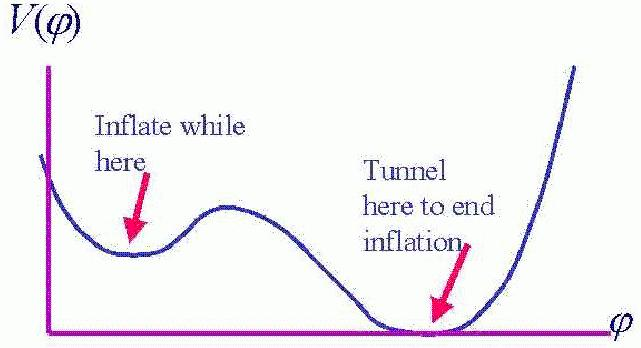
\includegraphics[width=0.5\linewidth, height=0.24\textheight]{Images/Chap2/GuthInflation_Fig5}
	\caption{Guth's potential in the old inflation. The inflation is achieved when the inflaton field is trapped in the false vacuum \cite{Chap2:Fig1}. }
	\label{fig:guthinflationfig5}
\end{figure}

Then, with a good appriximation, we can rewrite the energy density $ (\ref{Chap2EnergyDensity}) $ as 
\begin{equation}
	\label{Chap2:NewEnergyDensity}
	\rho(T)=\frac{\pi^{2}}{30}g_{*}(T)T^{4} + \rho_{0},
\end{equation}
where the value of $ \rho_{0} $ is positive and is determined by the particle theory.\\
We can rewrite (\ref{Chap2:Friedmann-Temperature}) as
\begin{equation}
\label{Chap2:Temperature-EnergydensityModified}
\Big(\frac{\dot{T}}{T}\Big)^{2}=\frac{4\pi^{2}}{45}Gg_{*}(T)T^{4}+\frac{8\pi G}{3}\rho_{0}.
\end{equation}
When the temperature is low enough the $ \rho_{0} $ term dominates over the other term in the RHS of the equation, and one has

\begin{equation}
	T(t)\simeq const \times e^{-\xi t}
\end{equation} 

where 

\begin{equation}
	\label{Chap2:psi}
	\xi^{2} =\frac{8\pi G}{3}\rho_{0}.
\end{equation}

Suppose that this supercooling continues down to some temperature $ T_{s} $, many orders of magnitude below $ T_{c} $.
Since from (\ref{Chap2:Friedmann-Temperature}) we have $ aT=const $, we finally obtain
\begin{equation}
	\label{Chap2:Expansion}
	a(t)=const \times e^{\xi t}.
\end{equation}
The universe is expanding exponentially, in a false vacuum state of energy density $\rho_{0}$.\\ In other words: if we consider initially the universe in thermal equilibrium (at least locally, in some regions), then when the temperature of such regions falls below $ T_{c} $ the effective potential of the inflaton field changes and at least another minimum  of the potential appears (true vacuum). However, the inflaton initially remains in the false vacuum and we have inflation.\\  
The universe will continue to supercool as it expands. Suppose that this cooling continues down to some temperature $ T_{s} $, many orders of magnitude below $ T_{c} $. When the field passes from the false vacuum to the true vacuum (by means quantum tunneling or in a classical way), the system undergoes a phase transition of the first order by means the generation of bubbles. When finally the phase transition takes place at $ T_{s} $ the latent heat is released and the universe is reheated at some temperature comparable to $ T_{c} $. We have the reheating stage.\\ 
As the universe expands and cools through the critical temperature $ T_{c} $ we have a nucleation of bubbles caused by the tunneling of the inflaton field from the false vacumm to the true one. The bubbles form randomly and we can introduce a certain nucleation rate $ \lambda(t) $, which is the probability per (physical) volume per time that a bubble will form in any region which is still in the high-temperature phase. We can imagine that the bubbles start at a point and expand at the speed of light. 
The crucial issue of this picture is that to solve the horizon and flatness problems the nucleation rate $ \lambda(t) $ needs to be slow compared to the expansion rate of the universe. This leads to disastrous consequences.\\
First af all, the latent heat released as a bubble expands is transferred initially to the walls of the bubble. This energy can be thermalized only when the bubbles walls undergo many collisions. As time goes on, we obtain regions of the universe occupied by separated clusters of these bubbles that grow in size. The range of these bubbles is immense. However, in these regions the clusters do not join together to form an infinite region (\textit{percolation}). It can be shown that the system percolates for large values of $ \lambda/\xi^{4} $, but for sufficiently small values it does not.\\
Without a sufficient collision of these bubbles we obtain an extremely dishomogeneous universe, far away from the current observations.

\subsection{Chaotic Inflation}
Consider a theory of a scalar field $\phi$ with effective potential $ V(\phi)=V_{0} = const > 0$. There are no reasons to expect that the classical field $\phi$ is equal to any particular value (e.g. $\phi = 0$) in the entire early universe. Instead, we expect that all values of the field $\phi$ may appears in different regions, with equal probability, varying from  $ -\infty $ to $ +\infty $ in different points of the universe. This is the idea of the \textit{Chaotic Inflation} \cite{ChaoticInflationLinde:Chap2}.\\
The only constraint we assume on the field $\phi$ in the early universe is that $ (\partial_{\mu} \phi)^{2} \le M_{P}^{2} $ for $ \mu = 0,1,2,3 $, since otherwise the corresponding part of the universe would be in the pre-planckian era, in which the classical description is impossible.\\
For example we can study the simplest model of a scalar field $\phi$ with a mass $ m $ and with the potential energy density $ V(\phi) = \frac{m^{2}}{2}\phi^{2} $ (fig. \ref{fig:chaoticinflationgwfrominflationfig3}).
\begin{figure}
	\centering
	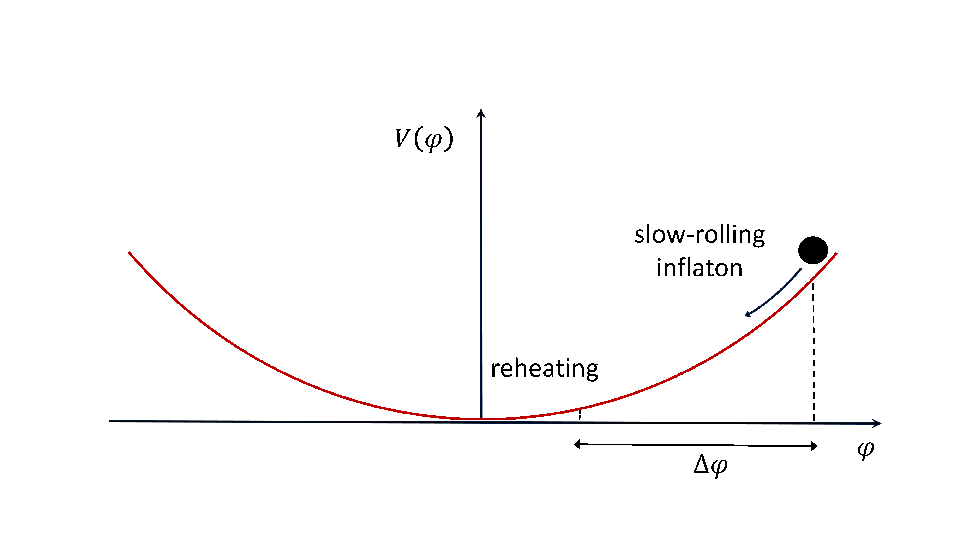
\includegraphics[width=0.55\linewidth, height=0.24\textheight]{Images/Chap2/ChaoticInflation_GWFromInflation_Fig3}
	\caption{Example of chaotic inflation potential. $ \Delta \phi $  indicates the inflaton excursion between the horizon exit of a given comoving scale and the end of inflation. Chaotic inflation is an example of \textit{large-field models} \cite{GWFromInflation:Intro}.}
	\label{fig:chaoticinflationgwfrominflationfig3}
\end{figure}
 Accountig for the expansion of the universe with Hubble constant $ H=\dot{a}/a $, the system is described by the equation of motion of the field $\phi$
\begin{equation}
	\label{Chap2eomChaoticInflation}
	\ddot{\phi} + 3H\dot{\phi} = -m^{2}\phi. 
\end{equation}
As said, the second term in the LHS of this equation can be interpreted as a friction term. The Friedmann equation (\ref{friedmannEquations1Chap2}) for a homogeneous universe containing the scalar field $\phi$ yields

\begin{equation}
	\label{Chap2:friedmannChaoticInflation}
	H^{2}=\frac{8 \pi G}{3}\rho_{\phi}= \frac{4 \pi G}{3}\Big (\dot{\phi}^{2} + m^{2}\phi^{2} \Big )
\end{equation}
where we have used (\ref{energyDensityPressure}) and neglected the curvature term.\\
From the last equation we see that if the scalar field $\phi$ initially was large, the Hubble parameter $ H $ had to be large too and then the friction term. This means that the scalar field during inflation was moving very slowly, as a ball in a viscous liquid. Therefore the energy density of the inflaton, unlike the density of ordinary matter, remained almost constant, and the expansion of the universe continued with a high speed. \\
Soon after the beginning of this regime (rapid expansion of the universe and slow motion of $\phi$) we obtain $ \ddot{\phi} \ll 3H\dot{\phi} $, $\dot{\phi^{2}}$ $\ll$ $ m^{2}\phi^{2} $, yielding
\begin{equation}
	\label{Chap2:HubbleRateField}
	H=\frac{\dot{a}}{a} =\sqrt{\frac{4\pi G}{3}}m\phi.
\end{equation}
 This equation shows that if the field $\phi$ changes slowly the size of the universe in this regime grows approximately as $ e^{H t} $ with $ H $ given by (\ref{Chap2:HubbleRateField}). \\
 In this model inflation does not require initial state of thermal equilibrium, supercooling and tunnelling from the false vacuum. This means that, in this scenario, there is no bubble nucleation and then the problems seen with Guth's model are avoided.\\
 When inflation ends, the scalar field $\phi$ begins to oscillate near the minimun of $ V(\phi) $. As any rapidly oscillating classical field, it looses its energy by creating pairs of elementary particles. These particles interact with each other and come to a state of thermal equilibrium with some temperature $ T_{r} $. From this time on, the universe can be described by the usual big bang theory.\\
 To have an idea of the huge expansion of the universe during inflation we can consider the mass $ m $ of the inflaton about $ 10^{-6} M_{p} $ and an initially closed universe with initial size $ l \simeq M_{p}^{-1} $. Moreover, we assume as initial condition for the energy density $\rho \simeq 1$ of the scalar field. From $\rho < 1$ we can consider this domain as classical universe.\\
 Solving (\ref{Chap2:HubbleRateField}) comes out that the total amount of inflation achieved starting from $ V(\phi) \simeq 1 $ is of the order of $ 10^{10^{10}} $ ! . In this model the total duration of inflation is about $ 10^{-30} $ seconds. From investigations of this period, if we consider the initial size of the universe small as the Planck size $ l_{p} $ $\simeq 10^{-33} cm$, after $ 10^{-30} $ seconds of inflation the universe acquires a huge size of $ l \simeq 10^{10^{10}} cm $ \cite{Chap2:Linde_HystoryInflation}. This value is model dependent, but in all realistic models  the size of the universe after inflation appears to be many orders of magnitude greater than the size of the part of the universe which we can see now, $ l \simeq 10^{28} cm $. Thus, most of the problems of the old cosmological theories are immediatly solved. \\
 If the universe initially consisted of many domains with chaotically distributed scalar field $\phi$, then domains with a value of the inflaton too small never inflated. Thus, the main contribution is given by those domains which originally contained large scalar field $\phi$. Inflation of such domain creates very large homogeneous islands out of initial chaos, each one much greater than the size of the observable part of the universe.\\
 Other examples of models of chaotic inflation are based on polynomial potentials. The first potential proposed by Linde, when he suggested the chaotic inflation scenario, was $ V(\phi) = \frac{\lambda}{4} \phi^{4} $ \cite{ChaoticInflationLinde:Chap2}. However, the main idea of this type of inflation is quite generic. One can consider any particular potential $ V(\phi) $, polynomial or not, with or without spontaneous symmetry breaking, and study all possible initial conditions without assuming that the universe was in a state of thermal equilibrium, and that the field $\phi$ was in the minimun of its effective potential from the very beginning.
 
 \subsection{Small-field models}
 The small field models are characterized by the following potential around $\phi=0$:
 \begin{equation}
 	\label{Chap2:small-field1}
 	V(\phi) = V_{0}\Big [1-\Big (\frac{\phi}{\mu}\Big)^{n} \Big]
 \end{equation}
which may arise in spontaneous symmetry breaking.
An important example is \textit{Natural Inflation} model where a Pseudo Nambu-Goldstone boson (PNGB) playes the role of inflaton \cite{Chap2:NaturalInflation}. The PNGB potential is in  the form
\begin{equation}
	\label{Chap2:PNGBPotential}
	V(\phi) = \Lambda^{4}\big [1 + cos(\phi/f) \big],
\end{equation}  
 where the two mass scales $\Lambda$ and $ f $ characterize the height and width of the potential, respectevely (fig. \ref{fig:naturalinflationinflationdynamics-and-reheating}). The potential has a unique minimun at $ \phi = \pi f $. The typical mass scales for successful inflation are of order  $ f \sim M_{pl} \sim 10^{19} $ Gev and $ \Lambda \sim m_{GUT} \sim 10^{16} Gev $. For temperatures $ T \le f $ the global symmetry is spontaneously broken. These mass scales arise in particle physics models, for example in superstring theories. \\
 \begin{figure}
 	\centering
 	\includegraphics[width=0.5\linewidth, height=0.25\textheight]{"Images/Chap2/NaturalInflation_InflationDynamics and reheating"}
 	\caption{Natural inflation potential. This is an example of \textit{small-field model} \cite{InflationDynamicsAndReheating:chap1}.}
 	\label{fig:naturalinflationinflationdynamics-and-reheating}
 \end{figure}
 
 We can describe the evolution of the field as 
 \begin{equation}
 	\label{Chap2:eomSmallFieldModel}
 	\ddot{\phi} + 3H\dot{\phi} + \Gamma\dot{\phi} + V'(\phi) = 0,
 \end{equation}
 
where $\Gamma$ is the decay rate of the inflaton.\\
When the temperature T $\le$ $\Lambda$, in regions of the universe with $\phi$ initially near the top of the potential, the field starts to slowly roll down toward the minimun of the potential. In those regions, the energy density of the universe is quickly dominated by the vacuum contribution and the universe expands exponentially. The slow-roll regime is characterized,  as in the previous models, by $ \ddot{\phi} \ll 3H\dot{\phi} $ and the initial condition for the field $\phi$, as in chaotic scenario, are random. \\
At the end of the slow-roll regime we have the reheating phase. The field $\phi$ begins to oscillate about the minimun of the potential, and gives rise to particle and entropy production. .
During this process the energy of the inflaton is converted in radiation in a time $\simeq \Gamma^{-1}$. If $\Gamma > H$, then the reheating process takes less than an expansion time ($\simeq H^{-1}$), and the coherent field energy is efficiently converted to radiation, reheating the universe to a temperature \cite{Chap2:NaturalInflation_Turner_Steinhardt}
\begin{equation}
\label{Chap2:ReheatingTemperatureSmallFieldModel}
T_{RH}=\Big (\frac{45}{4\pi^{3}g_{*}}\Big )^{1/4} (Hm_{pl})^{1/2}
\end{equation}
where $ g_{*} $ counts the effective number of relativistic degree of freedom.\\
On the other hand, if $ \Gamma < H $, then the reheating process takes longer than an expansion time. Until $ t \simeq \Gamma^{-1} $ the field continues to oscillate about the minimun of the potential. When $ t \simeq \Gamma^{-1} $ these oscillations are damped (in a few expansion times), reheating the universe to a temperature
\begin{equation}
	T_{RH} \simeq \Big (\frac{45}{4\pi^{3}g_{*}}\Big)^{1/4}(\Gamma m_{pl})^{1/2}.
\end{equation}

The decay rate can be evaluated as 
\begin{equation}
	\label{Chap2:DecayRate}
	\Gamma \simeq g^{2}\Lambda^{6}/f^{5}
\end{equation}
where g is an effective coupling constant (for example, in the axion model \cite{Chap2:AxionModel}, $ g \propto \alpha_{EM} $ for two-photon decay). For $ f=m_{pl} $ and $ g_{*}=10^{3} $, we find that $ T_{RH} \simeq 10^{14}\ Gev $ in the first case ($ \Gamma > H $) and $ T_{RH} \simeq 10^{8} g\ Gev$ in the other case ($\Gamma < H$). Since generally we expect that $ g < 1 $, the reheating temperature will be $ T_{RH} < 10^{8}\ Gev $ \cite{Chap2:NaturalInflation}.\\
This can have very insteresting application in GUT baryogenesis models (see \cite{Chap2:NaturalInflation} and \cite{Chap2:NaturalInflation_Turner_Steinhardt}).

\subsection{Hybrid models}
In this type of model the inflation ends because of the combination of several scalar fields. In particular, we have a scenario with two interacting scalar fields where inflation ends by a rapid rolling (\textit{waterfall}) of a second scalar field $\sigma$ besides the inflaton, triggered by the slow rolling of the field $\phi$ \cite{Chap2: Hybrid_Model}.\\
An example of effective potential from this type of model is given by
\begin{equation}
\label{Chap2:Hybrid model}
	V(\sigma,\phi) = \frac{1}{4\lambda}(M^{2}-\lambda \sigma^{2})^{2} + \frac{m^{2}}{2}\phi^{2} + \frac{g^{2}}{2}\phi^{2}\sigma^{2} 
\end{equation} 
When the fields have large value their effective mass squared are both positive and the potential has the symmetry $ \sigma \leftrightarrow -\sigma $. The potential has a maximum at $\phi = \sigma = 0$ and a global minimum at $\phi = 0$, $\sigma=\sigma_{0}=M/\sqrt{\lambda }$ where the symmetry is broken.\\
The effective mass squared of the field $\sigma$ is obtained by deriving the potential two times with respect the field $\sigma$:
\begin{equation}
	\label{massEffectiveSigma}
	m^{2}_{\sigma} = V''_{\sigma}(\sigma,\phi) = -M^{2} + g^{2}\phi^{2}.
\end{equation}
 Since the curvature of the effective potential in the $\sigma$-direction is much greater than in the $\phi$-direction we expect that at the first stages of expansion of the universe the field $\sigma$ rolled down to $\sigma=0$, whereas the field $\phi$ could remain large for longer time. Thus, we can consider the motion starting at large $\phi$ (where the effective mass of the $\sigma$ field is large) and the field is sitting at the minimum of the potential at $\sigma=0$.\\
 During the slow-roll of the field $\phi$, the effective mass of the triggering field is $ m^{2}_{\sigma} = g^{2}\phi^{2}-M^{2}$. As soon as the field $\phi$ acquires the critical value $\phi_{c}=M/g$, fluctuations of the massless $\sigma$ field trigger the symmetry breaking phase and inflation ends. \\
 \begin{figure}
 	\centering
 	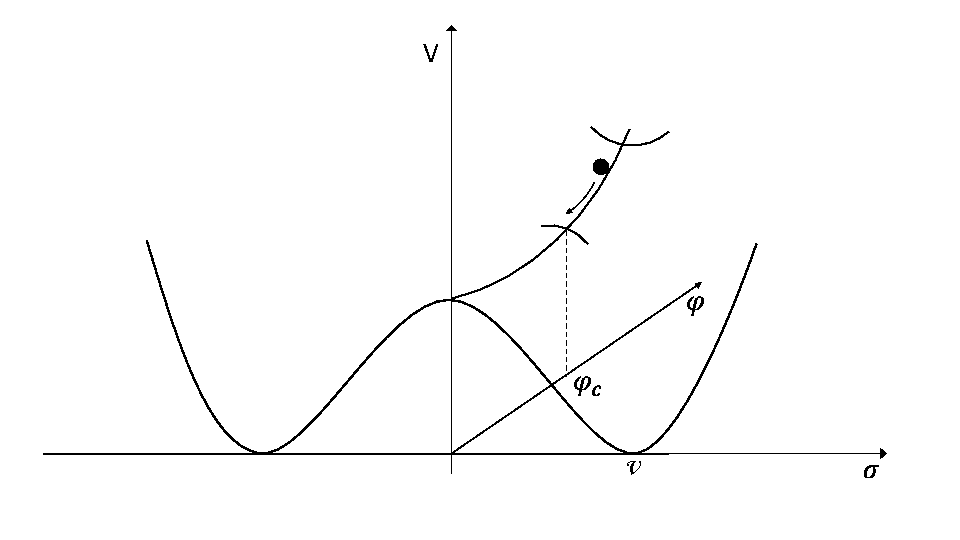
\includegraphics[width=0.55\linewidth, height=0.25\textheight]{Images/Chap2/HybridModel_GWFromInflation_Fig4}
 	\caption{Hybrid inflation potential. The field rolls down the potential up to the critical value $\phi_{c}$, and then reaches the true minimum of the potential $ \phi=0,\sigma=\sigma_{0}=v$ \cite{GWFromInflation:Intro}}
 	\label{fig:hybridmodelgwfrominflationfig4}.
 \end{figure}
 
 If the bare mass $ M $ is large compared with the rate of expansion $H$ of the universe, the transition will be instantaneous and inflation will end very rapidly. Instead, if the $ M $ parameter is of the order of $ H $, then the transition will be very slow and we can have a few more e-folds of inflation after the phase transition. When $ \sigma=0 $ the effective potential becomes
 \begin{equation}
 \label{effectivePotential}
 V(\phi)=\frac{M^{4}}{4\lambda} +  \frac{m^{2} \phi^{2}}{2}.
 \end{equation}
Since during inflation the scalar field $\phi$ is of the order $\phi_{c}=M/g$, if $ m^{2} \ll g^{2}M^{2}/\lambda $ we obtain for the potential the expression
\begin{equation}
	\label{potential}
	V(\phi,0)=\frac{M^{4}}{4\lambda} +  \frac{m^{2} \phi^{2}}{2} \simeq \frac{M^{4}}{4\lambda},
\end{equation} 
and for the Hubble rate, under this condition,
\begin{equation}
	\label{Chap2:HubbleHybrid}
	H^{2}\simeq\frac{8\pi G}{3} V(\phi,0) \simeq \frac{8\pi }{3M_{pl}^{2}}\frac{M^{4}}{4\lambda} =\frac{2\pi M^{4}}{3\lambda M_{pl}^{2}.}
\end{equation}
This means that, under the condition $  m^{2} \ll g^{2}M^{2}/\lambda $, we obtain inflation for $ \phi > \phi_{c} $. In this case the inflation is driven by the vacuum energy density $ V(0,0) = M^{4}/4\lambda $.\\
The complete equation of motion of the field $\phi$ is
\begin{equation}
	\ddot{\phi} + 3H\dot{\phi}=-(m^{2} + g^{2}\sigma^{2})\phi.
\end{equation}
As said, during inflation $\sigma=0$ and one can neglect $\ddot{\phi}$ in the equation of motion for the field $\phi$, yielding
\begin{equation}
	\label{eom}
	3H\dot{\phi}=-m^{2}\phi.
\end{equation}
It is then possible to integrate the evolution equation of $\phi$, obtaining
\begin{equation}	
	\label{Chap2:solutionField}
	\phi(N)=\phi_{c}e^{rN}, \qquad r\simeq \frac{m^{2}}{3H^{2}}
\end{equation}
where $ N=H(t_{c}-t) $ is the number of e-folds to the phase transition.\\
We can study the beheaviour of the field $\phi$ and $\sigma$ after the time 
$ \Delta t = H^{-1}=\sqrt{\frac{3\lambda}{2\pi}}\frac{M_{pl}}{M^{2}} $ from the moment $ t_{c} $ when the field $\phi$ becomes equal to $\phi_{c}$.
Considering the equation of motion of the field during inflation (\ref{eom}), during the time $\Delta t$ the variation $\Delta \phi$ is
\begin{equation}
	\label{Chap2:variationDeltaPhi}
	\Delta \phi = \frac{m^{2} \phi_{c}}{3H^{2}} = \frac{m^{2}M}{3H^{2}g} = \frac{\lambda m^{2}M_{pl}^{2}}{2\pi gM^{3}}.
\end{equation}

Thus, the value of the field after $\Delta t$ becomes
\begin{equation}
	\label{Chap2:fieldSquare}
	\phi_{t_{c}-\Delta\phi}=\frac{M}{g}\Big (1-\frac{\lambda m^{2} M^{2}_{pl}} {2\pi M^{4}} \Big ).
\end{equation}
Moreover, after $ t_{c} - \Delta t $ the value of the negative mass squared of the field $\sigma$ (\ref{massEffectiveSigma}) becomes
\begin{equation}
	\label{Chap2}
	m^{2}_{\sigma} = - M^{2}(\phi) = - \frac{\lambda m^{2}M^{2}_{pl}}{\pi M^{2}} 
\end{equation}
where the square of the field $\phi$ is obtained expanding the square of (\ref{Chap2:fieldSquare}) (we are working in the regime $ M^{2} \gg \lambda m^{2}/g^{2} $).\\
The value of $ M^{2}(\phi) $ is much greater than $ H^{2} $ for $ M^{3} \ll \lambda m M_{pl}^{2} $ (see (\ref{Chap2:HubbleHybrid})). This means that the field $\sigma$ within the time $\Delta t \sim H^{-1} $ rolls down to its minimum at $\sigma (\phi) = M(\phi)/\sqrt{\lambda}$, rapidly oscillates near it and loses its energy  due to the expansion of the universe.\\
It can be checked that the field $\phi$ rolls down very fast towards the minimum of its effective potential within a time much smaller than $ H^{-1} $ if $ M^{3} \ll \sqrt{\lambda}gmM_{pl}^{2} $.\\
Thus, under these conditions inflation ends in this theory almost instantaneously, as soon as the field $\phi$ reaches the critical value $\phi_{c} = M/g$.\\
Considering the reheating phase at the end of this type of model it will be important the following consideration. According to the classical equation of motion, the field $ \sigma=0 $ cannot change its value because the first derivative of the effective potential at $\sigma=0$ vanishes. The spontaneous symmetry braking  in this case occurs due to the exponential growth of quantum fluctuations. Indeed, writing the (negative) effective mass squared of the field $ -m^{2}_{\sigma}(\phi)=g^{2}(\phi-\phi_{c}) $ we immediately see that it vanishes at the critical point, but becomes large and grows up to $ m^{2}_{\sigma}(0) = M $ as the field $\phi$ slides towards $\phi=0$. This leads to a fast growing of quantum fluctuations of the scalar field $\sigma$, producing an inhomogeneous distribution of the field $\sigma$ with $ <\sigma>=0 $. We'll return to this in a more detailed way later. \\
Quantum fluctuations of the inflaton field produce metric perturbations $ \mathcal{R} \simeq H\delta\phi/\dot{\phi} $, where $\delta \phi$ is the amplitude of the field fluctuations when they cross outside the Hubble scale.
Appying (\ref{PR}) with the solution (\ref{Chap2:solutionField}) we obtain
\begin{equation}
\dot{\phi}=-(Hr\phi_{c})e^{rN},	
\end{equation}
and 
\begin{equation}
	\label{Chap2:P_{R}}
	P_{\mathcal{R}}=\Big (\frac{H^{2}}{4\pi^{2}r^{2}\phi_{c}^{2}}\Big)e^{-2rN} = \frac{1}{r^{2}}\frac{g^{2}M^{2}}{6\pi\lambda M_{pl}^{2}}e^{-2rN}.
\end{equation}

However, another more accurate way to compute this spectrum (\ref{Chap2:P_{R}}) is in \cite{Chap2:PerturbationsHybridInflation}. The only difference is that the spectrum (\ref{Chap2:P_{R}}) is multiplied by $ C(r)^{2} $ where $ C(r)=\Gamma[3/2-r]/2^{r}\Gamma[3/2] $ $\simeq 1$ in the limit $ m\ll H $.
Moreover, \cite{Chap2:PerturbationsHybridInflation} evaluated the spectral tilt as
\begin{equation}
	n_{\mathcal{R}} - 1 = \frac{d\ ln\ P_{\mathcal{R}}}{d\ ln\ k} = 2r. 
\end{equation}
Note that the tilt is always greater than one in this model.\\
The hybrid inflation is also a version of the chaotic inflation scenario. The main difference between this scenario and the simplest versions of the one-field chaotic inflation is in the way inflation ends. In the theory with  a single field, inflation ends when the potential of this field becomes steep. In the hybrid picture, instead, inflation ends due to the presence of another scalar field that triggers the waterfall.\\
Several extensions of this scenario became quite popular in the context of supergravity and string cosmology.

\section{Observations}
Inflation is not just an interesting theory  that can resolve many problems of the standard Big-Bang cosmology. The inflation paradigm made several predictions which can be tested by cosmological observations.\\
The first important prediction is that the universe must be flat and in most models $ \Omega = 1 \pm 10^{-4} $.\\
 An other important prediction is that  inflationary perturbations generated during a slow-roll regime with $\epsilon,\eta$ $\ll 1$ have a nearly flat spectrum with $ n_{S}$ close to 1. In general the spectrum of inflationary perturbations usually is slightly non-flat. It is possibile to construct models with $ n_{S}$ extremely close (or even exactly equal) to 1, but the small deviation of the spectrum from the exact flatness is one of the distinguishing features of inflation.\\
 Perturbations of the metric could be scalar, vector or tensor. Inflation mostly produces scalar perturbations, but it also produces tensor perturbations with nearly flat spectrum, and it does not produce vector perturbations. As seen in the first chapter  there are important relations between the scalar and tensor perturbations produced by inflation.\\
 The perturbations coming from inflation produce specific peaks in the spectrum of CMB radiation.\\
 It is possible to violate each of these predictions if one makes inflationary theory sufficiently complicated. For example, it is possible to produce vector perturbations of the metric in the models where cosmic strings are produced at the end of inflation, which is the case of some other models of hybrid inflation. However, it is difficult to do so, and most of the inflationary models obey the predictions above \cite{Chap2:Linde_HystoryInflation}.\\
 The most recent constraints on inflation comes from the 2018 $ Planck $ measurements of the CMB anisotropies \cite{Chap2:Planck2018}. The \textit{Planck} mission estimates the spectral index as
 \begin{equation}
 	\label{spectral index}
 	n_{s}= 0.9626 \pm 0.0057  \qquad (68\% C.L.).
 \end{equation}
and the curvature constraint
 \begin{equation}
 	\label{curvatureConstraint}
 	\Omega_{K}= -0.011 \pm 0.013 \qquad  (95\% C.L).
 \end{equation}
Moreover, assuming that the tensor-to-scalar ratio $ r $ satisfies the consistency relation  ($ n_{T} = -r/8 $), combining \textit{Planck} temperature, low-\textit{l} polaritation, and lensing it is estimated
\begin{equation}
	r_{0.02} < 0.10 \qquad (95\% C.L.),
\end{equation}
where this quantity it is evaluated at the pivot scale $ k_{0}=0.02 $ $ Mpc^{-1} $.
To characterize the system we can write the power spectra w.r.t a pivot scale $ k_{0} $ as power laws
\begin{equation}
	\Delta_{T}(k) = \Delta_{T}(k_{0})\Big (\frac{k}{k_{0}}\Big)^{n_{T}} \qquad \Delta(k) = \Delta_{\zeta}(k_{0})\Big (\frac{k}{k_{0}}\Big)^{n_{s}-1}
\end{equation}
obtaining a set of 4 observables: 2 spectral indeces and 2 amplitudes.\\
Assuming the consistency relation true we can reduce the DOF to 3.  Exploiting the normalitation of CMB anisotropies on large angular scales $ \Delta T/T \sim 10^{-5}$ \cite{Chap2:Wilkinson}, one can constraint one of the two amplitudes since it contains both $\zeta$ and GW contributions.
From experimental constraints on amplitudes and spectral indeces we can also constraint  the slow-roll parameters since $ n_{T}=-2\epsilon $ and $ n_{S}-1=2\eta - 6\epsilon $.\\
The usually chosen DOF to classify inflationary models are taken to be $ (r,n_{s}) $, from which we build the parameter space.\\
In the $ (r,n_{s}) $ plane, we have that different classes of models (small-field, large-field, hybrid models) occupy different regions. Indeed, we can consider  the parameter $\eta\simeq M_{pl}V''/V$ and rewriting the tensor-to-scalar ratio in terms of the slow-roll parameters as $r=16\epsilon$ we obtain


\begin{equation}
	r(n_{s},\eta)=\frac{8}{3}(1-n_{s}) + \frac{2}{3\pi}M_{pl}^{2}\frac{V''}{V}.
\end{equation}
For $\eta < 0 $ we have small-field models, for $ 0<\eta<2\epsilon $ we have  large-field models and hybrid models provide $\eta>2\epsilon $. The hybrid models are almost excluded by observation yielding $ n_{s} \le 1 $.
As mentioned, even if we are considering only the simplest models which realise inflation, there is still a large variety of them ("zoology"). In addition, one can see that the large field models tend to produce more gravitational waves than small ones.
\begin{figure}
	\centering
	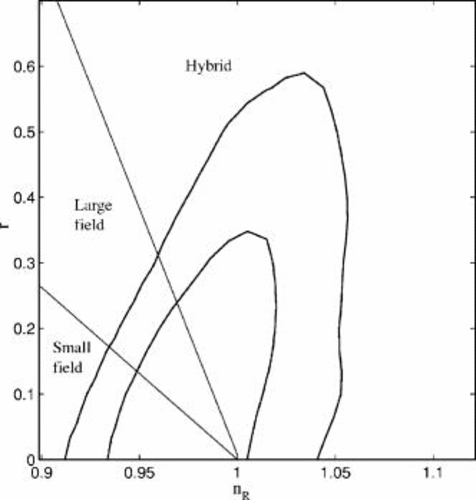
\includegraphics[width=0.6\linewidth, height=0.3\textheight]{Images/Chap2/r_ns_InflDynamicsAndReheating}
	\caption{Classification of inflationary models in the $ n_{\mathcal{R}}-r $ plane. The line $ r = (8/3)(1-n_{\mathcal{R}}) $ marks the border of large-field and small-field models,  whereas  the border of large-field and hybrid models correspond to $ r=8(1-n_\mathcal{R}) $ \cite{InflationDynamicsAndReheating:chap1}.}
	\label{fig:rnsinfldynamicsandreheating}
\end{figure}



\section{Reheating}
In this section we start to discuss one of the main focus of this thesis: The reheating stage after inflation.\\
As said, after  inflation the standard FLRW  radiation dominated universe should start, in order to recover the standard Big-Bang model of the universe. However, during the accelerated expansion of the universe $ T \propto a^{-1} \simeq e^{-Ht} $. Then, at the end of inflation the temperature becomes too small to allow a good thermalitation of the particles and then start the radiation dominated era. This is the reason why we need a post-inflation period in which the universe is reheated and which comes just before the radiation dominated era.\\
For now, we present a toy, elementary model of reheating. From Chapter 4 we'll investigate deeply such period and we will see, actually, that this phase leads to very interesting non-linear physics and dynamics. For reference see \cite{Chap2:Kolb_Turner}.\\
We start considering the simple single-field model discussed in the first chapter
\begin{equation}
		\mathcal{L} = -\dfrac{1}{2} g^{\mu\nu} \partial_{\mu}\phi \partial_{\nu} \phi - V(\phi).
\end{equation}	
Inflation ends when the slow-roll parameter $\epsilon$ reaches the value 1, which implies that also $\eta=1$. Indeed, this happens when the curvature $ V'' $ of the potential stars to become non negligible, implying that the flat region in which the slow-roll takes place has ended. This stage is equivalent to say that $ V''\sim H^{2} $, that means $\eta \sim 1$ from (\ref{eta2}) (we recall that we have renaimed $\eta_{V}$ as $\eta$). \\
From this moment the second derivative of the potential starts to increase, becoming greater than the rate of the expansion of the universe, and the inflaton begins to oscillate around the minimun with an high frequency $\omega$. This leads to $ V'' \propto \omega^{2} \gg H^{2} $.
Moreover, the inflaton not only starts to oscillate with high frequency around the minimum of the potential but it also decays with a rate $\Gamma_{\phi}$ to lighter relativistic particles that reheat the universe.\\
We can then modify the equation of motion for the inflaton field in a way that takes into account its decay
\begin{equation}
	\label{Chap2:EOM_Modified}
	\ddot{\phi} + (3H + \Gamma_{\phi})\dot{\phi} + V'(\phi) = 0.
\end{equation}
We remark that the decay rate is a rate such as $H  $  and then they should be multiplied by $\dot{\phi}$.\\
Consider now the energy density of the inflaton $\rho_{\phi} = \frac{1}{2} \dot{\phi^{2}} + V(\phi)$ and compute the time derivative
\begin{equation}
	\label{Chap2:dotPhi}
	\dot{\rho_{\phi}}=\dot{\phi}\ddot{\phi} + V'\dot{\phi}.
\end{equation}
Multiplying (\ref{Chap2:EOM_Modified}) by $\dot{\phi}$ and using the last expression, we obtain
\begin{equation}
	\label{Chap2:dotPhiEquation}
	\dot{\rho_{\phi}} + \dot{\phi^{2}}(3H^{2} + \Gamma_{\phi}) = 0
\end{equation}
Moreover, using the fact that the typical time of oscillation is much smaller than the characteristic time of expansion, we can take an average over a period of oscillation such as
\begin{equation}
	\label{Chap2:oscillationAverage}
	\dfrac{1}{2} <\dot{\phi^{2}}>_{period}\ =\ <V(\phi)>_{period}\qquad \rightarrow\qquad \rho_{\phi}\ =\ <\dot{\phi^{2}}>_{period}
\end{equation}
Finally, the final form of (\ref{Chap2:dotPhiEquation}) reads
\begin{equation}
	\label{Chap2:FinalEqRho}
\dot{\rho}_{\phi} + (3H + \Gamma_{\phi})\rho_{\phi} = 0	.
\end{equation}
To solve this equation we consider the general solution
\begin{equation}
	\label{Chap2:rhoSolution1}
	\rho_{\phi}(t)=\rho_{osc}e^{-A(t)}, \qquad A(t)=\int_{t_{osc}}^{t}(3H+\Gamma_{\phi})dt
\end{equation}
where $ \rho_{osc} $ denotes the initial condition at $ t_{osc} $, the time at which the inflaton begins to oscillate. The solution for $ A(t) $ reads
\begin{equation}
	\label{Chap2:solutionAt)}
	A(t)= \int_{t_{osc}}^{t}\Big (3 \frac{\dot{a}}{a} + \Gamma_{\phi}\Big) dt = 3 \ln \Big(\frac{a(t)}{a_{osc}}\Big) + \Gamma_{\phi}(t-t_{osc})
\end{equation}
and, substituing in (\ref{Chap2:rhoSolution1}), we finally obtain the solution
\begin{equation}
\label{Chap2:rhoSolution}
\rho_{\phi} = \rho_{osc} \Big (\frac{a}{a_{osc}}\Big)^{-3}e^{-(t-t_{osc})\Gamma_{\phi}}.	
\end{equation}
From this equation we obtain an interesting feature of this system: during the oscillation phase the inflaton beheaves as non-relativistic pressureless matter. Moreover, we can impose as initial condition $ \rho_{osc}=M^{4} $.
The exponential extra factor accounts for the decay of the field.\\
We can summarize the situation. After the end of inflation, as a consequence of the no-more negligible curvature of the potential, the inflaton field moves towards the minimum and starts to oscillate around it with an high frequency. At times $ t $ near to $ t_{osc} $ the decay of $\phi$ is not efficient and $\rho_{\phi}$ decreases essentially as $ a^{-3} $. However, the field $\phi$ starts to decay, with a rate $\Gamma_{\phi}$. Because of these contributions the energy density of the inflaton decreases, but still dominates the energy density of the universe. As time passes, the decay starts to become important and  at $ t_{decay} \sim 1/\Gamma_{\phi} $ becomes very efficient.
At this point the energy density of the inflaton starts to be very strongly suppressed and that of the relativistic particles increases.\\
The presence of the new term $\Gamma_{\phi}$ related  to the decay of the inflaton field brings to a modification also to the equation for the energy density of radiation, which becomes
\begin{equation}
	\label{Chap2:radiationEquation}
	\dot{\rho_{r}} + 4H\rho_{r} = \Gamma_{\phi}\rho_{\phi}.
\end{equation}
As we said, from $ t_{osc} \simeq H^{-1} \simeq M_{pl}/M^{2} $ to $ t_{decay} \simeq \Gamma^{-1} $ the field oscillates but, although in principle it can decay, this process is still not efficient. Lighter particles begin to be produced in a slow way and their energy is still dominated by that of the inflaton, which energy continues to decrease.\\
As a consequence of this peculiar phase $\rho_{r}$ has not the particular beheaviour $ a^{-4} $ which is expected from the standard radiation dominated era, but the universe is still dominated by a matter-like field. In such phase the scale factor evolves as $ a \propto t^{2/3} $ and the Hubble constant reads $ H=2/3t $.\\
Thus, starting from (\ref{Chap2:radiationEquation}) we can write
\begin{equation}
	\label{Chap2:radiationEquation2}
	\dot{\rho_{r}} + \frac{8}{3t}\rho_{r}\simeq \Gamma_{\phi}\rho_{osc}\Big (\frac{a}{a_{osc}}\Big)^{-3}
\end{equation}
where we have evaluated the expression near $ t_{osc} \sim M_{pl}/M^{2} $, neglecting the exponential term in $\rho_{\phi}$. Considering the time beheaviour of the scale factor  and $\rho_{osc}=M^{4}$ this equation yields
\begin{equation}
	\label{Chap2:radiation3}
		\dot{\rho_{r}} + \frac{8}{3t}\rho_{r} \simeq \Gamma_{\phi} M^{4} \Big (\frac{t}{t_{osc}}\Big)^{-2} \simeq \frac{\Gamma_{\phi} M_{pl}^{2}}{t^{2}}
\end{equation}
To solve this equation we can search solution for $ \rho_{r} \propto t^{\alpha} $, taking as initial condition $\rho_{r}(t_{osc})=0$. We can use also the general solution
\begin{equation}
	\label{Chap2:generalSolution}
	\rho_{r}(t)=c_{in}e^{-A(t)} + e^{-A(t)} \int_{t_{osc}}^{t}dt'\ (g(t')e^{A(t')}), \qquad 
	g(t') = \frac{\Gamma_{\phi} M_{pl}^{2}}{t'^{2}}  
\end{equation}
where $ c_{in} $ denotes the initial condition. Putting $ \rho(t_{osc})=0 $ it is easy to see that $ c_{in}=0 $. The $ A(t) $ term is given by
\begin{equation}
	\label{Chap2:A(t)2}
	A(t)=\int_{t_{osc}}^{t}\frac{8}{3t'}dt'=\frac{8}{3}\ln(t/t_{osc})
\end{equation}
Finally, the integral term in (\ref{Chap2:generalSolution}) yields
\begin{equation}
	\label{Chap2:IntegralTerm}
	\int_{t_{osc}}^{t} dt'\frac{\Gamma_{\phi} M_{pl}^{2}}{t'^{2}}\Big (\frac{t'}{t_{osc}}\Big)^{8/3} = \frac{9}{40}\frac{\Gamma_{\phi} M_{pl}^{2}}{t_{osc}^{8/3}}(t^{5/3} - t_{osc}^{5/3})
\end{equation}
Putting all inside (\ref{Chap2:generalSolution}) we obtain
\begin{equation}
	\rho_{r}=\frac{9}{40}\frac{\Gamma_{\phi}M_{pl}^{2}}{t}\Big (1- \Big (\frac{t}{t_{osc}}\Big)^{-5/3}\Big)
\end{equation}
Using the scaling beheaviour $ a \propto t^{2/3} $ we can write the last expression in terms of the scale factor, obtaining the final solution
\begin{equation}
\label{Chap2:finalSolution}
\rho_{r}(t)=\frac{9}{40}\frac{\Gamma_{\phi}M_{pl}^{2}}{t_{osc}}\Big (\frac{a}{a_{osc}}\Big)^{-3/2}\Big (1- \Big (\frac{a}{a_{osc}}\Big)^{-5/2}\Big)
\end{equation}
and, using $ t_{osc}=M_{pl}/M^{2} $
\begin{equation}
	\rho_{r}(t)=\frac{9}{40}\Gamma_{\phi}M_{pl}M^{2}\Big (\frac{a}{a_{osc}}\Big)^{-3/2}\Big (1- \Big (\frac{a}{a_{osc}}\Big)^{-5/2}\Big)
\end{equation}
From this equation we can determine easily the beheaviour of the radiation energy density. During the period of oscillation of the inflaton field the radiation energy starts to grow from zero up to a maximum value $\rho_{max} \simeq \Gamma_{\phi} M_{pl} M^{2}$ thanks to the inflaton decays. Once the maximum is reached, $\rho_{r}$ decreased as $ a^{-3/2} $, instead of the usual $ a^{-4} $.\\
Regarding the temperature we can estimate the maximum temperature reached by the radiation fluid at $\rho_{max}$ using $ \rho_{r}=(\pi^{2}/30)g_{*}T^{4} $. We obtain 
\begin{equation}
	T_{max} \sim g_{*}^{-1/4}(\rho_{r}^{max})^{1/4} \sim g_{*}^{-1/4}\Gamma_{\phi}^{1/4}M_{pl}^{1/4}M^{1/2}.
\end{equation}
During this phase the system  is still between the start of oscillations and the time at which decays become efficient. In such period we have that also the entropy increases. Indeed, the total entropy $ S = sa^{3} $ is constant only if the entropy density scales as $ s \propto a^{3} $. This happens only in a pure FLRW radiation dominated universe and we are not yet in that phase.\\
In this period 
\begin{equation}
\label{Chap2:entropy}
s \propto T^{3} \sim \rho_{r}^{3/4} \sim a^{-9/8}
\end{equation}
that leads
\begin{equation}
	\label{Chap2:totalEntropy}
	S \propto a^{15/8}.
\end{equation}
Thus, during this stage the inflaton decays producing new relativistic particles and this process causes the increasing of the entropy.\\
In the final stage we reach the time $ t_{decay} \sim \Gamma^{-1}_{\phi} $. From this moment the decay of the inflaton is efficient due to the exponential term in (\ref{Chap2:rhoSolution}). The energy density of the field $\rho_{\phi}$ decreases rapidly and $\rho_{r}$ becomes the dominant energy density allowing to recover the usual radiation dominated era in which $ \rho_{r} \propto a^{-4} $ and $ S=const $. The temperature at which the radiation energy becomes the dominant energy of the universe (and then the radiation dominated era begins) is called \textit{Reheating Temperature} $ T_{R} $. To estimate this temperature we can consider the Hubble constant during the standard radiation dominated era, and evaluating it at $ t_{decay}=\Gamma_{\phi}^{-1} $:
\begin{equation}
	\label{HubbleConstant}
	H^{2} = \Big (\frac{1}{2t}\Big)^{2} = \frac{\Gamma_{\phi}^{2}}{4} 
\end{equation}
and,
\begin{equation}
	H^{2}=\frac{8\pi }{3M_{pl}^{2}}\rho_{r}\simeq \frac{8 \pi g_{*}}{3M_{pl}^{2}}\frac{\pi^{2}}{30}T^{4}_{\ |t\simeq \Gamma_{\phi}^{-1}}.
\end{equation}
Combining the last two equations we finally derive an estimate of the reheating temperature
\begin{equation}
	\label{Chap2:reheatingTemperature}
	T_{R} \simeq 0.55g_{*}^{1/4}(\Gamma_{\phi}M_{pl})^{1/2}.
\end{equation}
where we assumed for semplicity that the radiation dominated era starts at the instant $ t_{decay} $, when the decay of the inflaton field becomes efficient.\\ 
As final comment we notice that there is no remnant of the vacuum energy density of the inflaton field, which drives the accelerated expansion of the universe. Indeed, just after inflation $\phi$ beheaves as a non-relativistic pressureless field which causes its redshifting as $ a^{3} $.\\
There is also a special case in which the reheating is istantaneous at $ \rho_{osc} \simeq M^{4} \simeq T^{4}_{R} $. This happens when at $ t_{osc} $ the decay of the inflaton field is already extremelly efficient. $\phi$ will not even make a single oscillation around the minimun transformig immediately all the vacuum energy directly into radiation. In this special case we have $ T_{R} \simeq M $.



\chapter{Gravitational Waves and Other Observables}

\chapter{Preheating}

\chapter{Other models of Preheating}

\chapter{Non Linear Evolution After Preheating: Bubbly Stage}

\chapter{Thermalitation}

\chapter{Gravitational waves and Reheating}

\chapter{Other Signatures of Reheating}

\begin{thebibliography}{2}
	
	\bibitem{Liddle:intro} A. R. Liddle and D. H. Lyth, \emph{Cosmological inflation and large-scale structure} (Cambridge University Press, 2006).
	
	\bibitem{NonGauss:Intro} N. Bartolo, E. Komatsu, S. Matarrese and A. Riotto, Phys. Rept. \textbf{402}, 103 (2004) [arXiv:astro-ph/0406398].
	
	\bibitem{GWFromInflation:Intro} M. C. Guzzetti, N. Bartolo, M. Liguori and S. Matarrese, (2016), arXiv:1605.01615. 
	
	\bibitem{Guth:Intro} A. Guth, Phys. Rev. \textbf{D23}, 347 (1981) .
	
	\bibitem{COBE1:intro} K. M. G´orski, et al. Astrophys. J. \textbf{464}, L11 (1996) [arXiv:astro-ph/9701191].
	
	\bibitem{COBE2:intro} G. F. Smoot, et al., Astrophys. J. \textbf{396}, L1 (1992).

    \bibitem{WMAP:intro} H. V. Peiris, et al., Astrophys. J. Suppl. \textbf{148}, 213 (2003).
	
	\bibitem{Planck2018:intro} Y. Akrami et al., Astron. Astrophys. \textbf{641}, A9 (2020).
	
	\bibitem{Steigman:nucleosynthesisIntro} G. Steigman, Ann.Rev.Nucl.Part.Sci. \textbf{57}, 463-491 (2007) [arXiv:0712.1100].
	
	\bibitem{ReheatingPredictionsSingleFieldModel:intro} J.L. Cook et al., JCAP \textbf{1504} (2015) 047 [arXiv:1502.04673].
	
	\bibitem{Bicep2:Intro} BICEP2, Keck Array, P.A.R. Ade et al., Phys. Rev. Lett. \textbf{116}, 031302 (2016) [arXiv:1510.09217].
	
	\bibitem{Bicep2BMode:Intro} BICEP2 Collaboration, P. Ade et al., Phys. Rev. Lett. \textbf{112} (2014) 241101 [arXiv:1403.3985].
	
	\bibitem{COre:intro} COrE, F. R. Bouchet et al., (2011), arXiv:1102.2181.  
	
	\bibitem{PRISM:intro} PRISM, P. Andrè et al., JCAP \textbf{1402}, 006 (2014) [arXiv:1310.1554].
	
	\bibitem{LIGO:intro} LIGO Scientific, J.Aasi et al., Class. Quant. Grav. \textbf{32} (2015) 074001 [arXiv:1411.4547].
	
	\bibitem{Lisa:Intro} A. Klein et al., Phys. Rev. \textbf{D93}, 024003 (2016) [arXiv:1511.05581].
	
	\bibitem{InflationDynamicsAndReheating:chap1} B. A. Bassett, S. Tsujikawa and D. Wands, Rev. Mod. Phys. \textbf{78}, 537 (2006) [arXiv:astro-ph/0507632].
	
	\bibitem{Dodelson:Chap1} S. Dodelson, F. Schmidt, \emph{Modern Cosmology} (Academic Press, 2020).
	
	\bibitem{TopDefects:Linde} A. Linde,  (1990), arXiv:hep-th/0503203.
	
	\bibitem{Plank2015:Chap1} Planck, P. A. R. Ade et al., (2015), arXiv:1502.02114.
	
	\bibitem{Chap2:Fig1} A. Albrecht, (2000), arXiv:astro-ph/0007247.
	
	\bibitem{Chap2: Linde_NewInflation} A. D. Linde, Phys. Lett. \textbf{B108}, 389 (1982).
	
	\bibitem{ChaoticInflationLinde:Chap2} A. D. Linde, Phys. Lett. \textbf{B129}, 177  (1983).  
	
	\bibitem{Chap2:Linde_HystoryInflation} A. Linde, (2007), arXiv: 0705.0164. 
	
	\bibitem{Chap2:NaturalInflation} K. Freese, J. A. Frieman and A. V. Olinto, Phys. Rev. Lett. \textbf{65}, 3233 (1990).
	
	\bibitem{Chap2:NaturalInflation_Turner_Steinhardt} P. J. Steinhardt and M. S. Turner, Phys. Rev. \textbf{D29}, 2162 (1984).
	
	\bibitem{Chap2:AxionModel} J. E. Kim, Phys. Rep. \textbf{150}, 1 (1987).
	
	\bibitem{Chap2: Hybrid_Model} A. Linde, (1993), arXiv: astro-ph/9307002.
	
	\bibitem{Chap2:PerturbationsHybridInflation} J. Garcìa-Bellido, A. D. Linde and D. Wands, Phys. Rev. \textbf{D54}, 377 (1996).
	
	\bibitem{Chap2:Planck2018} Planck Collaboration, Astron. Astrophys. \textbf{641}, A10 (2020).
	
	\bibitem{Chap2:Wilkinson} H. V. Peiris \textit{et al.}, Astrophys. J. Suppl. \textbf{148}, 213 (2003) [arXiv:astro-ph/0302225].
	
	\bibitem{Chap2:Kolb_Turner} E. W. Kolb, M. S. Turner, \textit{The Early Universe} (Westview Press, 1994).
	
	
		
\end{thebibliography}	
	
\end{document}
